% The document class supplies options to control rendering of some standard
% features in the result.  The goal is for uniform style, so some attention 
% to detail is *vital* with all fields.  Each field (i.e., text inside the
% curly braces below, so the MEng text inside {MEng} for instance) should 
% take into account the following:
%
% - author name       should be formatted as "FirstName LastName"
%   (not "Initial LastName" for example),
% - supervisor name   should be formatted as "Title FirstName LastName"
%   (where Title is "Dr." or "Prof." for example),
% - degree programme  should be "BSc", "MEng", "MSci", "MSc" or "PhD",
% - dissertation title should be correctly capitalised (plus you can have
%   an optional sub-title if appropriate, or leave this field blank),
% - dissertation type should be formatted as one of the following:
%   * for the MEng degree programme either "enterprise" or "research" to
%     reflect the stream,
%   * for the MSc  degree programme "$X/Y/Z$" for a project deemed to be
%     X%, Y% and Z% of type I, II and III.
% - year              should be formatted as a 4-digit year of submission
%   (so 2014 rather than the academic year, say 2013/14 say).


\documentclass[ % the name of the author
                    author={Tengyao Tu},
                % the name of the supervisor
                supervisor={Dr. James Pope},
                % the degree programme
                    degree={MSc},
                % the dissertation    title (which cannot be blank)
                     title={A New Perspective on Graph Community Detection: Combining Traditional Methods with Deep Learning Approaches},
                % the dissertation subtitle (which can    be blank)
                  subtitle={Applying to Telecom Networks and Diverse Datasets},
                % the dissertation     type
                      type={},
                % the year of submission
                      year={2024}]{dissertation}
%基本算法包


\usepackage{amsmath} 
\usepackage{algorithmic}
\usepackage{tcolorbox}
\renewcommand{\thealgorithm}{\arabic{chapter}.\arabic{algorithm}}
\errorcontextlines\maxdimen
% Define a new tcolorbox environment for algorithms with a box around it
% Define a new environment for framing the algorithm
\newtcolorbox[auto counter, number within=chapter]{framedalgorithm}[2][]{%
    colback=white!10!white, colframe=black,
    fonttitle=\bfseries,
    title=Algorithm~\thetcbcounter: #2,#1
}



\begin{document}

\maketitle

% =============================================================================

% This section simply introduces the structural guidelines.  It can clearly
% be deleted (or commented out) if you use the file as a template for your
% own dissertation: everything following it is in the correct order to use 
% as is.


% After the title page (which is a special case in that it is not numbered)
% comes the front matter or preliminaries; this macro signals the start of
% such content, meaning the pages are numbered with Roman numerals.



\frontmatter

% This macro creates the standard UoB declaration; on the printed hard-copy,
% this must be physically signed by the author in the space indicated.

\makedecl

% LaTeX automatically generates a table of contents, plus associated lists 
% of figures, tables and algorithms.  The former is a compulsory part of the
% dissertation, but if you do not require the latter they can be suppressed
% by simply commenting out the associated macro.

\tableofcontents
\listoffigures
\listoftables
\listofalgorithms

% The following sections are part of the front matter, but are not generated
% automatically by LaTeX; using \chapter* means they are not numbered.

% -----------------------------------------------------------------------------

\chapter*{Abstract}
Graph community detection is essential in modern network science and graph machine learning. It can identify a group of nodes with tight internal connections and sparse external connections. It has been widely and successfully applied in various fields, such as interest groups in social networks, content clustering in recommendation systems, functional module recognition in protein networks, and financial security analysis. In applying telecom graphs, graph community detection also plays a significant role. Firstly, it can help identify user interest communities, thereby assisting telecommunications companies in building recommendation systems. Secondly, it can accurately detect base station faults, helping telecommunications companies save costs. However, how to detect accurate and commercially meaningful communities, as well as how to detect communities quickly, have become challenges for community detection on large-scale telecom graphs. 

Most current community detection approaches are divided into four types: Hierarchical Clustering Algorithm, Modularity Optimization Algorithm, Random Walk-Based Clustering Algorithm, and Machine Learning-Based Clustering Algorithm. Among them, the Louvain algorithm based on modularity optimization has been widely applied due to its low time complexity and good performance. However, this algorithm only relies on the structural information of the graph and cannot include the features of nodes and edges. Machine learning algorithms can effectively combine the feature information of nodes and edges for detection, but the training time is long, and the performance is unstable.

Our dissertation proposes a hybrid community detection algorithm, \textbf{Louvain-Enhanced GNN Clusternet (LEGC)}, that combines traditional and machine learning detection. LEGC uses the Louvain algorithm to obtain an initial community detection result, which is converted into a one-hot representation as an additional node attribute. After the message passes through GNN, Clusternet optimises graph embedding. The community detection results obtained in this way comprehensively consider the features of nodes and edges in the dataset. Moreover, since the features already contain initial partitions, it accelerates the optimisation process of Clusternet and improves its performance. 

For experimental rigour, we discuss the performance comparison of LEGC on datasets from multiple fields. LEGC performed significantly better than other scholars' existing work on multiple datasets. At the same time, we conduct detailed ablation experiments to demonstrate the significance of LEGC's innovative design. Finally, we discuss in detail the commercial applications of LEGC in telecommunications graphs and provide some practical suggestions.

The main contributions of our dissertation are as follows:
\begin{quote}
\noindent
\begin{itemize}
\item We proposed a novel community detection algorithm (LEGC) suitable for large-scale datasets, and we found that this algorithm significantly improves model performance and reduces model training time.
\item We used datasets from multiple fields (including paper citation networks, protein networks, and social networks) to demonstrate the rigour of the model and the performance of different methods on datasets of different scales.
\item We presented in detail the results of using LEGC for telecom graph community segmentation, fully demonstrating the application of community detection in enterprises.
\item We discussed using community detection to annotate unsupervised datasets.
\end{itemize}
\end{quote}



% -----------------------------------------------------------------------------

%\chapter*{Summary of Changes}

%{\bf A conditional section, of at most $1$ page} 
%\vspace{1cm} 

%If (and only if) the dissertation represents a resubmission (e.g., as the %result of
%a resit), then this section is compulsory: the content should summarise %all
%non-trivial changes made to the initial submission.  Otherwise you can
%omit it, since {\bf a summary of this type is only needed for %resubmissions}.

%When included, the section will ideally be used to highlight additional
%work completed, and address criticism raised in any associated feedback.
%Clearly it is difficult to give generic advice about how to do so, but
%an example might be as follows:

%\begin{quote}
%\noindent
%\begin{itemize}
%\item Feedback from the initial submission criticised the design and 
%      implementation of my genetic algorithm, stating ``there seems 
%      to have been no attention to computational complexity during the
%      design, and obvious methods of optimisation are missing within
%      the resulting implementation''.  Chapter 3 now includes a
%      comprehensive analysis of the algorithm, in terms of both time
%      and space.  While I have not altered the algorithm itself, I
%      have included a cache mechanism (also detailed in Chapter 3)
%      that provides a significant improvement in average run-time.
%\item I added a feature in my implementation to allow automatic rather
%      than manual selection of various parameters; the experimental
%      results in Chapter 4 have been updated to reflect this.
%\item Questions after the presentation highlighted a range of related
%      work that I had not considered: I have make a number of updates 
%      to Chapter 2, resolving this issue.
%\end{itemize}
%\end{quote}

% -----------------------------------------------------------------------------

\chapter*{Supporting Technologies}
\begin{quote}
\noindent
\begin{itemize}

\item I use Python as my main programming language.
\item I use PyTorch as my deep learning framework.
\item The datasets from SNAP and Pytorch-Geometric are used in our models.
\item I use Huawei Cloud Services as my computing hardware resource.
\item I used \LaTeX\ to format my thesis, via the online service {\em Overleaf}. 
\end{itemize}
\end{quote}

% -----------------------------------------------------------------------------

\chapter*{Notation and Acronyms}



\begin{quote}
\noindent
\begin{tabular}{lcl}
GNN                 &:     &  Graph Neural Network                                         \\
GCN                &:     &  Graph Convolutional Network                                         \\
GraphSAGE                &:     &  Graph Sample and Aggregation                                     \\
GAT                &:     &  Graph Attention Network                                    \\
GT                &:     &   Graph Transformer                                    \\
LEGC                 &:     & Louvain-Enhanced Graph Neural Network-Clusternet                                         \\
PCA                &:     &   Principal Component Analysis                                    \\
FA               &:     &    Factor Analysis                                    \\
t-SNE               &:     &    t-Distributed Stochastic Neighbor Embedding                                   \\
DG              &:     &     Dynamic Graph                                   \\
HG              &:     &     Heterogeneous Graph                                  \\
WG              &:     &     Weighted Graph                                  \\

NMI              &:     &     Normalized Mutual Information                                  \\
GAE              &:     &     Graph Autoencoder                                  \\
SOBI              &:     &     Service-Oriented  Business Intelligence                                \\
LIDE              &:     &     Local Information-based Deep Embedding                                 \\
SDNE              &:     &     Structural Deep Network Embedding                                 \\
DDGAE              &:     &      Deep Dual Graph
Attention Encoder                              \\
             &:     &                                    \\
Q              &:     &     \text{Modularity} \\
A_{ij}         &:     &     \text{Adjacency matrix entry }  \\
k_i            &:     &     \text{Degree of node } i \\
m              &:     &     \text{Total number of edges in the network} \\
\delta(c_i, c_j) &:     &     \text{1 if nodes } i \text{ and } j \text{ are in the same community, 0 otherwise} \\
D              &:     &     \text{Degree Matrix} \\
H^{(l)}        &:     &     \text{Feature matrix of the } l\text{-th layer, containing the features of nodes at layer } l \\
W^{(l)}        &:     &     \text{Weight matrix of the } l\text{-th layer, containing the learnable parameters of the layer} \\
N(v)           &:     &     \text{Set of nodes obtained by Neighbor Sampling for node } v \\
b^{(l)}        &:     &     \text{Bias of the } l\text{-th layer, used to adjust the output of the layer} \\
\alpha_{ij}    &:     &     \text{Attention weight between node } i \text{ and node } j \\
F_{\text{spring force}, ij}    &:     &     \text{Spring force between node } i \text{ and node } j \\
F_{\text{repulsive force}, ij} &:     &     \text{Repulsive force between node } i \text{ and node } j \\
F_{\text{friction}, ij}        &:     &     \text{Friction between node } i \text{ and node } j \\
F_{\text{gravity}, i}          &:     &     \text{Gravity of node } i \\
F_{\text{total}, i}            &:     &     \text{Total force on node } i \\
d_{ij}                         &:     &     \text{Distance between node } i \text{ and node } j \\
k, k_e, \beta, \tau, \gamma    &:     &     \text{Different constants used in force calculations} \\
l_0                            &:     &     \text{Ideal length of the spring} \\
\mathbf{r}_i                   &:     &     \text{Displacement vector from node } i \text{ to the center of gravity} \\

\end{tabular}
\end{quote}

% -----------------------------------------------------------------------------

\chapter*{Acknowledgements}

Completing my master's thesis marked the next stage of my life. First, I would like to express my gratitude to my family for their support, without which I would have had difficulty obtaining this master's degree. Second, I would like to thank my mentors James Pope and Tim Samogan from BT for their patient guidance, which has helped me a lot. Finally, I would like to thank everyone who has assisted me with the project.

The biggest enemy of learning is self-satisfaction, and I will continue to strive and surpass myself in my future studies and work.

% =============================================================================

% After the front matter comes a number of chapters; under each chapter,
% sections, subsections and even subsubsections are permissible.  The
% pages in this part are numbered with Arabic numerals.  Note that:
%
% - A reference point can be marked using \label{XXX}, and then later
%   referred to via \ref{XXX}; for example Chapter\ref{chap:context}.
% - The chapters are presented here in one file; this can become hard
%   to manage.  An alternative is to save the content in seprate files
%   the use \input{XXX} to import it, which acts like the #include
%   directive in C.

\mainmatter

% -----------------------------------------------------------------------------

\chapter{Introduction}
\label{chap:introduction}
This chapter first introduces the background of graph community detection and telecom graph applications. Then, we explain why graph community detection is an important research field. Next, we discuss the existing methods of graph community detection and their limitations. At the same time, we introduce the state-of-the-art models of graph community detection. Finally, we briefly describe our method, the main challenges, and research objectives.
\begin{figure}[h!] % 'h!' attempts to position the figure here
    \centering
    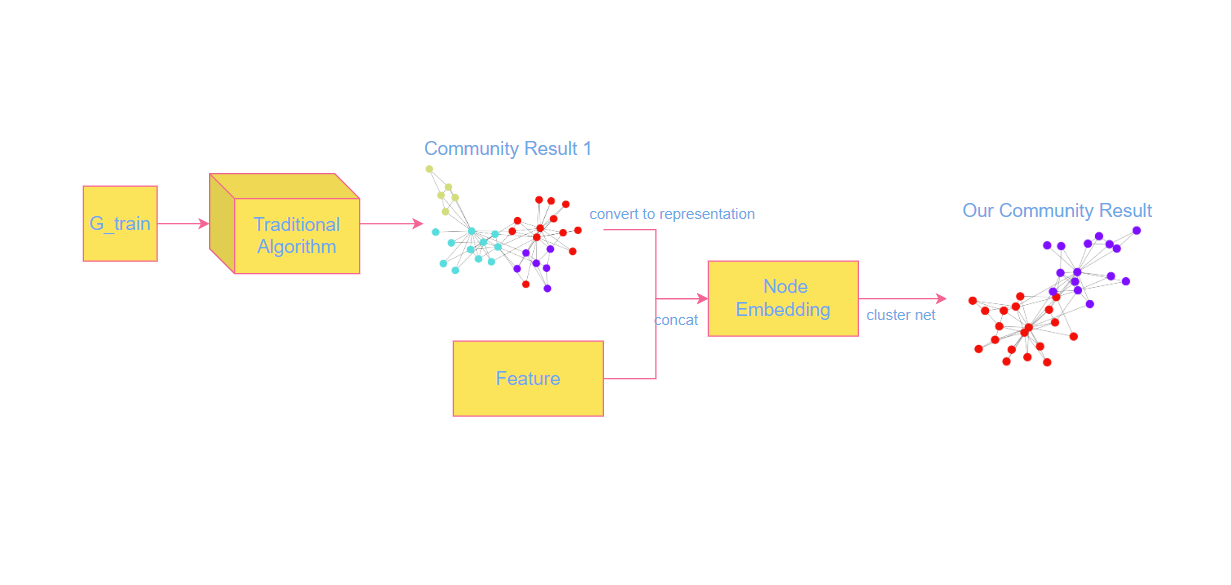
\includegraphics[width=1.0\textwidth]{Figure_2.png} % Adjust the width to scale the image
    \caption{The Top-level Design of The Approach (LEGC)}
    \label{fig: Our Approach}
\end{figure}

\section{Background}

With the popularisation of the Internet and the increasingly fierce competition in the telecommunications market, operators need to use business intelligence to provide more personalised services for different customers. However, popular methods nowadays focus on the customer, such as SOBI architecture~\cite{ishaya2012service} based on customer needs. This method is time-consuming and labour-intensive, especially for large telecommunications companies with many users and base stations, making it almost impossible to complete.

In network science~\cite{barabasi2013network}, if a group of nodes are tightly connected internally and sparsely connected externally, we can refer to this group of nodes as a community. Graph community detection is widely used in telecommunications graphs and is an essential technology for companies to enhance their competitiveness.
\section{Motivations}
Based on the above background, our project is the application of graph community detection in telecommunications graphs.
\subsection{Introduction to Graph Community Detection}
After Watts and other scholars~\cite{watts1998collective} proposed the small world network model, modern network science entered a new stage of development. Graph machine learning has also made significant breakthroughs and achievements in the past decade~\cite{xia2021graph}.

Graph community detection~\cite{fortunato2010community} is a hot research topic in modern network science and graph machine learning. In social networks, detecting communities can serve as an essential criterion for recommendation systems~\cite{bedi2016community}.In bioinformatics, community detection can identify key modules of biological processes (protein networks~\cite{manipur2021community}).In sociological research, community detection can help identify interaction patterns among different social groups~\cite{solomon2019understanding}. At the same time, community detection has also achieved high success in financial fraud~\cite{li2022internet}, network security~\cite{chen2022mobile}, and market analysis~\cite{rahimnezhad2020application}.

In telecommunications networks, graph community detection also plays a significant role. Firstly, it can analyse user behaviour patterns and serve as new business intelligence to provide customers with more personalised services and packages. Secondly, it can help identify abnormal behaviour in the network and quickly isolate the faulty area when a fault occurs~\cite{he2020fault}. Thirdly, it can optimise the traffic configuration of operators and allocate different bandwidth resources to different communities~\cite{yuan2024huawei}.

Unlike graph partitioning, community detection aims to reveal the inherent community structure of the network. The number and size of communities are not specified in advance and must be discovered after checking the network connection patterns. However, the time complexity of the exhaustive method is $O(2^n)$(\( n \) is the number of nodes). Therefore, implementing simple and efficient community detection algorithms is also the topic we will discuss next.
\subsection{Current Approaches}
Next, we will review existing community detection algorithms based on literature and explain their advantages and disadvantages.
\subsubsection{Hierarchical Clustering Algorithm}
Hierarchical clustering is one of the earliest community detection algorithms, which can be divided into agglomerative algorithm(e.g. Ravasz algorithm~\cite{ravasz2002hierarchical}) and divisive algorithm(e.g. Girvan-Newman algorithm~\cite{newman2004finding}). The algorithm using Ravasz's algorithm as an example is shown in Algorithm 1.1.
\begin{algorithm}[ht!]
\caption{Ravasz's algorithm} 
\begin{framedalgorithm}[ht!]
    \State \textbf{Input} Graph $G$\newline
    \State \textbf{Output} Tree Diagram of All Nodes\newline
   \State \textbf{Initialize} each node as its own community $C_{i}$\newline
    \State \textbf{Initialize} similarity $S_{ij}$ for all pairs of nodes $(i, j)$\newline
    \State \textbf{While} $|C| > 1$\textbf{do}\newline
    \State \phantom{hold} Merge the two communities with the highest similarity $S_{ij}$\newline
    \State \phantom{hold}Recalculate the similarity $S_{ij}$ for all pairs of communities\newline
    \State \textbf{End While}\newline
\end{framedalgorithm}
\end{algorithm}
According to Algorithm 1.1, the time complexity of hierarchical clustering is $O(N^2)$. This is much more efficient than an exhaustive search. However, for large-scale graphs, the time complexity is still too high, and hierarchical clustering has a certain degree of ambiguity, as it does not determine which partition is optimal. So, hierarchical clustering is not suitable for large-scale graphs; it is now suitable for situations that require flexible partitioning of the number of clusters~\cite{li2019community}. Next, we will discuss other community detection algorithms.
\subsubsection{Modularity Optimization Algorithm}
The critical indicator for evaluating community division is \textbf{Modularity}, and the modularity calculation is elaborated in detail in Chapter 2 of the article. The first modular optimization algorithm(FN) was proposed by Mark Newman~\cite{newman2004fast}. Subsequently, different scholars have made improvements to the algorithm (Louvain algorithm~\cite{blondel2008fast}, CNM algorithm~\cite{clauset2004finding}). However, they are all based on modularity optimization algorithms, which merge communities pairwise until modularity cannot be increased. The algorithm using the Louvain algorithm as an example is shown in Algorithm 1.2.
\begin{algorithm}[ht!]
\caption{Modularity Optimization Algorithm}
\begin{framedalgorithm}[ht!]
    \State \textbf{Input} Graph G \newline
    \State \textbf{Output} Community Partition $C$\newline
   \State \textbf{Initialize} each node as its own community $C_{i}$\newline
    \State \textbf{Initialize} modularity M\newline
    \State \textbf{While} $|C| > 1$\textbf{do}\newline
    \State \phantom{hold} Merge the two communities and calculate $\triangle M$\newline
    \State \phantom{hold} Record the largest M and its Partition $C$\newline
    \State \textbf{End While} \newline
\end{framedalgorithm}
\end{algorithm}
The time complexity of the CNM and Louvain algorithms is $O(N \log^2 N)$ and $O(N \log N)$, respectively. They are more suitable for community detection of large-scale graphs. In addition, Infomap~\cite{rosvall2008maps} and LPA~\cite{garza2019community} also have similar time complexity as Louvain.
\subsubsection{Random Walk-Based Clustering Algorithm}
In addition to the methods of detecting communities mentioned above, clustering graph embeddings to detect communities is another important approach. The quality of community detection is directly related to graph embedding vectors. The algorithm process is shown in Algorithm 1.3.
\begin{algorithm}
\caption{Graph Embedding Clustering Algorithm}
\begin{framedalgorithm}[ht!]
    \State \textbf{Input} Graph G and Features F\newline
    \State \textbf{Output} Community Partition $C$ and Node Embeddings $E$\newline
    \State \textbf{Initialize} Node Embedding $E$ by Any Methods\newline
    \State \textbf{Initialize} Cluster Center $N$\newline
    \State \textbf{Calculate} Community Partition $C$ based on Cluster Result \newline
\end{framedalgorithm}
\end{algorithm}
We can generate graph embedding vectors through random walks. Common methods include Deepwalk~\cite{perozzi2014deepwalk},Node2Vec~\cite{grover2016node2vec},Struc2Vec~\cite{ribeiro2017struc2vec}.
\subsubsection{Machine Learning-Based Clustering Algorithm}
The algorithm flow based on machine learning is also shown in Algorithm 1.3, with the only difference being how Node Embeddings are generated. Models that have succeeded greatly include LIDE~\cite{chou2019local}, SDNE~\cite{wang2016structural}, and others. The popular community detection methods nowadays are also based on machine learning methods. For example, DDGAE (2024)~\cite{wu2024deep},GNN (2024)~\cite{liu2024community},FBCD(2024)~\cite{liu2024community}, Graph Autoencoder(2024)~\cite{jie2024overlapping}.
\section{Our Approach}
We propose a novel machine learning-based community detection model that integrates traditional community detection algorithms with graph embedding techniques. We name this method as Louvain-Enhanced GNN Clusternet (LEGC). Our method detects more reasonable communities than traditional community detection algorithms. Later in the thesis, we will elaborate that high modularity community segmentation may not necessarily be the most reasonable segmentation. Meanwhile, compared to traditional machine learning algorithms, our method does not require too many training batches for convergence and has a faster convergence speed.

We use the features of the nodes themselves and traditional community detection results as the starting vectors for graph embedding, GCN~\cite{kipf2016semi}, GAT~\cite{velivckovic2017graph}, GraphSAGE~\cite{hamilton2017inductive}, Graph Transformer~\cite{yun2019graph} and their variants~\cite{zhu2020hgcn}~\cite{yang2021hgat}~\cite{hu2020heterogeneous} as encoders for graph embedding models, and VAGE~\cite{kipf2016variational} and Clusternet~\cite{wilder2019end} as decoders to train graph embedding vectors. Meanwhile, we compared other community detection algorithms. The details of our algorithm will be elaborated in Chapter 3. The top-level design of our method is shown in Figure 1.1.
\subsection{Research Aim}
To propose a new community detection algorithm, our aims are summarized as follows:
\begin{itemize}
\item Develop a community detection algorithm suitable for large-scale Telecom Graph data, providing insights into community detection for BT Research.
\item Explore the performance of different community detection algorithms and which are suitable for large-scale data.
\item Research whether using traditional community algorithms to enhance graph embedding vectors can improve machine learning algorithms' performance and training speed.
\item Compare the performance of different algorithms on different datasets.
\item Investigating whether graph community detection can label data and allow efficient and massively transformation of unsupervised datasets into supervised datasets.

\end{itemize}
\subsection{Challenges}
Our algorithm is a novel GNN method different from GPT-GNN~\cite{hu2020gpt}. There are four main concerns:
\begin{itemize}
\item The first concern is whether using traditional community detection algorithms to enhance machine learning models can improve the performance or training speed of the model, as the embedding vectors of the graph after adding pre-trained models become more complex.
\item The second concern is related to robustness. Our method may affect multiple datasets differently, and some may perform poorly.
\item The third concern is related to model design and parameter selection. Choosing the appropriate optimizer, training batch, and model structure requires more exploration.
\item The fourth concern is related to time costs. There may be a problem of long training time for community detection on large-scale graphs.

\end{itemize}
% -----------------------------------------------------------------------------

\chapter{Technical Background}
This chapter provides the technical background of the project, basic concepts of community and modularity (Sections 2.1 and 2.2), and force-oriented layout (Section 2.3). We introduce the graph neural network technology we used and discuss the advantages and disadvantages of various graph neural networks through mathematical formulas (Section 2.4). Finally, we briefly introduce the K-means algorithm (Section 2.5) and dimensionality reduction method (Section 2.6).  Through this chapter, we provide a theoretical foundation for Chapter 3.
\label{chap:background}
\section{Community}
For an undirected graph \( G = (V, E) \), where \( V \) is the set of vertices and \( E \) is the set of edges, the density \( D \) is defined as Formula 2.1:
\begin{equation}
D = \frac{|E|}{|V| (|V| - 1)}
\label{eq:directed_density}
\end{equation}
So, the meaning of a community in a graph is a subset C that has a higher density than the other parts of the graph, as shown in Formula 2.2:
\begin{equation}
   D_{C} \gg D_{C, \text{ext}}
\label{eq:community}
\end{equation}
After introducing the mathematical representation of the community, Figure 2.1 shows the communities of the Karate Club~\cite{zachary1977information}.
\begin{figure}[h!] % 'h!' attempts to position the figure here
    \centering
    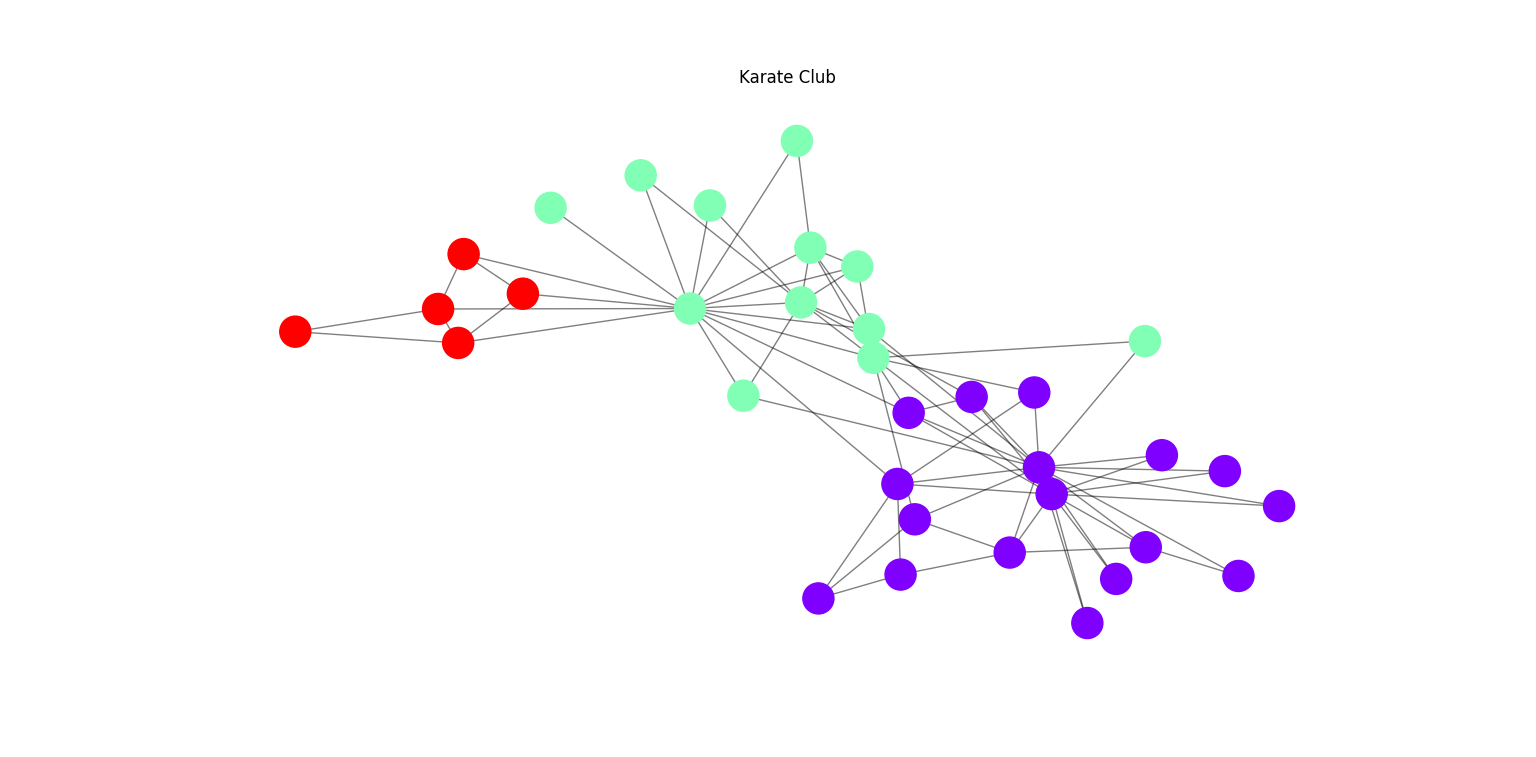
\includegraphics[width=0.9\textwidth]{Figure_1.png} % Adjust the width to scale the image
    \caption{Karate Club Graph's Communities}
    \label{fig: Karate Club graph's communities}
\end{figure}
This classic dataset showcases different communities very well. After introducing communities, we will introduce an important evaluation metric for community detection: Modularity.
\section{Modularity}
The definition of modularity has been elaborated in many articles~\cite{faraj2022community}~\cite{leicht2008community}, and its original definition is Formula 2.3.
\begin{equation}
Q = \frac{1}{2m} \sum_{ij} \left[ A_{ij} - \frac{k_i k_j}{2m} \right] \delta(c_i, c_j)
\label{eq:modularity}
\end{equation}
There are many variant formulas for modularity, and the modularity of \textbf{Directed Graph} is shown in Formula 2.4.
\begin{equation}
Q_d = \frac{1}{2m} \sum_{ij} \left[ A_{ij} - \frac{k_i^{\text{out}} k_j^{\text{in}}}{2m} \right] \delta(c_i, c_j)
\label{eq: directedmodularity}
\end{equation}
The modularity of \textbf{Dynamic Graph} is as Formula 2.5.
\begin{equation}
Q_t = \frac{1}{2m_t} \sum_{ij} \left[ A_{ij}(t) - \frac{k_i(t) k_j(t)}{2m_t} \right] \delta(c_i(t), c_j(t))
\label{eq: dynamicmodularity}
\end{equation}
The modularity of  \textbf{Weighted Graph} is as Formula 2.6.
\begin{equation}
Q_w = \frac{1}{W} \sum_{ij} \left[ w_{ij} - \frac{k_i k_j}{W} \right] \delta(c_i, c_j)
\label{eq: weightedmodularity}
\end{equation}
where:
\begin{itemize}
  \item $A_{ij}$ or $w_{ij}$ is the adjacency matrix entry.
  \item $k_i$ and $k_j$ are the degrees of nodes $i$ and $j$, respectively.
  \item $m$ or $W$ is the total number of edges in the graph.
  \item $\delta(c_i, c_j)$ is an indicator function that is 1 if nodes $i$ and $j$ are in the same community and 0 otherwise.
\end{itemize}
From formula (2.3), we can conclude that the community partitioning results are good when the modularity is close to 1. In contrast, when it is close to 0 or negative, it indicates poor community partitioning results, similar to or worse than random partitioning.
\section{Graph Visualization Based on Force-Directed Layout}
Graph visualisation is an essential step in graph community detection, as the detected community structure needs to be presented to everyone rather than just displaying seemingly ideal modularity data. The most common visualisation method is \textbf{Spatial Layout}, which means that when we know the spatial information of each node, we can directly use their spatial positions for layout.For example: Traffic Graph~\cite{shin2024pgcn},Geography Graph~\cite{wang2024hypergraph}.

For graphs without spatial information, we have Random Layouts, Hierarchical Layouts, Grid Layouts, Circular Layouts, and so on. However, these layouts have an inferior effect on large-scale graphs, and it is impossible to visualise the typical graph structure.

For large-scale graphs without geographical location, we use \textbf{Force-Directed Layout}, and its principle has been explained in multiple articles~\cite{hu2005efficient}~\cite{lin2012new}~\cite{kobourov2012spring}. Different scholars have different optimisation methods, and here we provide the calculation process of the CosmoGraph~\cite{cosmograph2024}(a variant of Force-Directed Layout) we use.
The formula for spring force is Formula 2.7.
\begin{equation}
F_{ij}^{\text{spring force}} = -k \cdot (d_{ij} - l_0)
\label{eq: springforce}
\end{equation}
The formula for repulsive force is Formula 2.8.
\begin{equation}
F_{ij}^{\text{repulsive force}} = \frac{k_e}{d_{ij}^2}
\label{eq: repulsizeforce}
\end{equation}
The formula for frictional force is Formula 2.9.
\begin{equation}
F_{ij}^{\text{friction}} = -\beta \cdot \frac{d_{ij}}{\tau}
\label{eq: frictionalforce}
\end{equation}
The formula for gravitational force is as Formula 2.10.
\begin{equation}
F_{i}^{\text{gravity}} = -\gamma \cdot \mathbf{r}_{i}
\label{eq: gravity}
\end{equation}
The formula for total force is Formula 2.11.
\begin{equation}
F_{i}^{\text{total}} = F_{ij}^{\text{spring force}}+F_{ij}^{\text{repulsive force}}+F_{ij}^{\text{friction}}+F_{i}^{\text{gravity}}
\label{eq: total}
\end{equation}
where:
\begin{itemize}
  \item $F_{ij}^{\text{spring force}}$ is the spring force between $node_i$ and $node_j$; $F_{ij}^{\text{repulsive force}}$ is the repulsive force between $node_i$ and $node_j$; $F_{ij}^{\text{friction}}$ is the friction between $node_i$ and $node_j$; $F_{i}^{\text{gravity}}$ is the gravity of $node_i$; $F_{i}^{\text{total}}$ is the total force of $node_i$.
  \item $d_{ij}$is the distance between $node_i$ and $node_j$.
  \item $k$, $k_e$, $\beta$, $\tau$ and $\gamma$ are different constants.
  \item $l_0$ is the ideal length of the spring.
  \item $r_i$ is displacement vector from $node_i$ to the center of gravity.
\end{itemize}
According to the above formula, we update the layout as shown in Algorithm 2.1.
\begin{algorithm}[ht!]
\caption{Force-Directed Layout}
\begin{framedalgorithm}[ht!]
    
    \State \textbf{Input} Initial Node Positions(random generated)\newline 
    \State \textbf{Output} Final Layout\newline
    \State \textbf{Initialize:} Randomly initialize node positions\newline
     \State \textbf{For} each pair of nodes $i$ and $j$ \textbf{do}\newline
     \State  \phantom{hold}\textbf{Compute} the total force $F_{ij}^{\text{total}}$ between nodes $i$ and $j$\newline
     \State \phantom{hold}\textbf{Update} node position \newline
     \State \textbf{Endfor}\newline
      \State \textbf{Iterate:} Repeat the  Calculation and Update steps until the system reaches a stable state\newline
\end{framedalgorithm}
\end{algorithm}
Our subsequent visualised telecom graph is based on Algorithm 2.1. It plays a vital role in visualising large-scale graphs. Many open-source tools such as Gephi~\cite{bastian2009gephi}~\cite{grandjean2015gephi}, Cytoscape~\cite{shannon2003cytoscape}, and Pajek~\cite{mrvar2020pajek} have achieved excellent visualisation of large-scale graphs based on Force-Directed Layout.
\section{Graph Neural Network}
Graph neural networks(GNN) are the most important technology we use, which learns on graph data through \textbf{Message Passing} mechanisms. Many scholars~\cite{wu2020comprehensive}~\cite{khemani2024review}~\cite{zhou2020graph} have provided a detailed review of graph neural networks, and we summarise their research to introduce the graph neural network models we use.
\subsection{Graph Convolutional Network(GCN)}
GCN updates node features by weighted averaging the features of neighbouring nodes, and its formula is shown in Formula 2.12.
\begin{equation}
H^{(l+1)} = \text{ReLU}\left(D^{-\frac{1}{2}} (A + I) D^{-\frac{1}{2}} H^{(l)} W^{(l)}\right)
\label{eq: GCN}
\end{equation}
where:
\begin{itemize}
  \item A is the adjacency matrix.
  \item I is the identity matrix to consider the characteristics of its nodes.
  \item D is the degree matrix.
  \item $H^{(l)}$ is the feature matrix of the l-th layer.
  \item $W^{(l)}$ is the weight matrix of the l-th layer.
\end{itemize}
Graph convolutional networks use standardised adjacency matrices and feature matrices to update features, which is simple and efficient. However, it has some drawbacks. Firstly, its weights are fixed. Secondly, it calculates the entire graph, and when the graph is vast, the computational workload is high or even impossible to calculate.
\subsection{Graph Sample and Aggregation(GraphSAGE)}
GraphSAGE effectively solves the computational complexity problem, divided into two steps: 1. Neighbor Sampling and 2. Aggregation. The formula for feature update is shown in 2.13.
\begin{equation}
H_v^{(l+1)} &= \sigma \left( W^{(l)} \cdot \text{AGGREGATE} \left( \{ H_u^{(l)} \mid u \in N(v) \} \right) + b^{(l)} \right)
\label{eq: GraphSAGE}
\end{equation}
where:
\begin{itemize}
  \item $H_v^{(l+1)}$ is the feature of node v in the l-th layer.
  \item $W^{(l)}$ is the weight matrix of the l-th layer.
  \item $N(v)$ is the set of nodes by Neighbor Sampling.
  \item $b^{(l)}$ is the bias of the l-th layer.
  \item \text{AGGREGATE} is the aggregation function (such as summation, averaging, maxpooling, LSTM~\cite{graves2012long}).
\end{itemize}
GraphSAGE is a flexible graph neural network that reduces computational burden through sampling and aggregation. However, selecting aggregation functions and sampling sizes can significantly affect GraphSAGE's performance, so its tuning process is complex.
\subsection{Graph Attention Network(GAT)}
In the message passing of GNN, the influence between nodes is not unique, and GCN standardises the influence between nodes through degrees. GAT considers this degree of influence as a learnable parameter(attention coefficient). The attention coefficient $\alpha_{vu}$ calculation is shown in Formula 2.14.
\begin{equation}
\alpha_{ij} = \text{softmax}\left( \text{LeakyReLU}\left( \mathbf{a}^T \left[ \mathbf{W} \mathbf{h}_i \| \mathbf{W} \mathbf{h}_j \right] \right) \right)
\label{eq: GAT}
\end{equation}
where:
\begin{itemize}
    \item $\alpha_{ij}$ is the attention weight of node i and node j.
    \item  $W$ is the weight matrix.
    \item  ${a}^T$ is the attention coefficient vector.
    \item  \text{LeakyReLU} is an activation function that, unlike ReLu, allows for a minimal linear value to occur in the negative interval.
    \item ${h}_i$ is the feature of node i.
\end{itemize}
The feature update method of GAT is shown in Formula 2.15.
\begin{equation}
\mathbf{H}_v^{(l+1)} = \sigma \left( \sum_{u \in \mathcal{N}(v)} \alpha_{vu} \mathbf{W} \mathbf{H}_u^{(l)} \right)
\label{eq: GAT2}
\end{equation}
Meanwhile, GAT can enhance expression ability through multi-head attention, as shown in Formula 2.16.
\begin{equation}
\mathbf{H}_v^{(l+1)} = \|_{k=1}^K \sigma \left( \sum_{u \in \mathcal{N}(v)} \alpha_{vu}^k \mathbf{W}^k \mathbf{H}_u^{(l)} \right)
\label{eq: GAT3}
\end{equation}
where:
\begin{itemize}
    \item K is the number of attention heads.
    \item ${W}^k$ is the weight matrix of the k-th attention head.
    \item $\alpha_{vu}^k$ is the attention coefficient of the k-th attention head.
\end{itemize}
GAT performs well, but storing attention matrices for large-scale graphs may result in higher memory usage. Moreover, we have found in reviews by other scholars that GAT is not as effective as GCN for global graph structure information.
\subsection{Graph Transformer(GT)}
Transformer~\cite{vaswani2017attention} is an essential neural network architecture that has fundamentally changed fields such as natural language processing(NLP)~\cite{devlin2018bert} and computer vision(CV)~\cite{kim2021vilt}.

Graph Transformer has also achieved outstanding results as a robust graph neural network architecture based on Transformer. Next, we will introduce the principle of Graph Transformer based on reviews from other scholars~\cite{min2022transformer}. Graph Transformer calculates attention score through the Self-Attention Mechanism, as shown in Formula 2.17. Next, calculate the attention weights as shown in Formula 2.18.
\begin{equation}
e_{ij} = \frac{(W_Q h_i)^\top (W_K h_j)}{\sqrt{d_k}}
\label{eq: Transformer1}
\end{equation}
\begin{equation}
\alpha_{ij} = \text{softmax}(e_{ij})
\label{eq: Transformer2}
\end{equation}

The calculation of the weighted features of nodes is shown in Formula 2.19.
\begin{equation}
H_i^{(l+1)}= \sum_{j \in \mathcal{N}(i)} \alpha_{ij} (W_V H_j^{(l)})
\label{eq: Transformer3}
\end{equation}
where:
\begin{itemize}
    \item $W_Q$ is the weight matrix of the Query(Q).
    \item $W_K$ is the weight matrix of the Key(K).
    \item $W_V$ is the weight matrix of the Value(V).
    \item $d_k$ is the dimension of the key.
\end{itemize}
Like GAT, Graph Transformer can also improve the expressive power of the model through a multi-head attention mechanism. Firstly, GT calculates the weighted features of each attention head, as shown in Formula 2.20.
\begin{equation}
H_i^{\text{head}_k} = \sum_{j \in \mathcal{N}(i)} \alpha_{ij}^k (W_V^k H_j)
\label{eq: Transformer4}
\end{equation}
Then, concatenate the outputs of all attention heads, as shown in Formula 2.21.
\begin{equation}
H_i^{\text{F}} = \text{CONCAT}(H_i^{\text{head}_1}, H_i^{\text{head}_2}, \ldots, H_i^{\text{head}_K}) W_O
\label{eq: Transformer5}
\end{equation}
where:
\begin{itemize}
    \item k is the k-th attention head.
    \item $W_V^k$ is the weight matrix of the k-th head.
    \item $W_O$ is the weight matrix of the Output(O).
\end{itemize}
GT uses Transformer architecture to calculate attention coefficients, which can capture global information and some long-range dependencies well, but the computation will be more complex.
\section{K-means clustering}
According to Algorithm 1.3, after obtaining the embeddings generated by GNN, we need to cluster the embeddings of the nodes to obtain the divided communities.Common clustering algorithms include K-means~\cite{burkardt2009k}, DBSCAN~\cite{deng2020dbscan},Gaussian Mixture Model~\cite{reynolds2009gaussian},Mean Shift~\cite{comaniciu2002mean}, Hierarchical clustering~\cite{nielsen2016hierarchical} and their variants.

Most scholars use k-means as the clustering algorithm in community detection algorithms. It is highly computationally efficient and suitable for large-scale graph data, and its convergence speed is usually the fastest. 

Moreover, K-means with soft allocation make it easier to implement backpropagation, thereby adjusting the values of graph embeddings and producing better results. This is also the difference between supervised graph tasks and unsupervised graph tasks. Supervised graph tasks use the cross entropy of predicted and accurate labels for backpropagation. In contrast, unsupervised graph tasks use the objective function obtained through the soft allocation of K-means for backpropagation. The process of K-means is shown in Algorithm 2.2.
\begin{algorithm}[ht!]
\caption{K-means Clustering}
\begin{framedalgorithm}[ht!]
    
    \State \textbf{Input} Data points $X = \{x_1, x_2, \ldots, x_n\}$, Number of clusters $K$, Number of iterations $T$\newline 
    \State \textbf{Output} Final cluster centroids $C = \{c_1, c_2, \ldots, c_k\}$, Community Partition $D$\newline
    \State \textbf{Initialize:} centroids $C = \{c_1, c_2, \ldots, c_k\}$ randomly\newline
    \State \textbf{For} iteration $t = 1$ \textbf{to} $T$\newline
    \State \phantom{hold}\textbf{For} each data point $x_i$ \textbf{do}\newline
    \State \phantom{hold}\textbf{Assign} $x_i$ to the nearest centroid $c_j$ based on Euclidean distance\newline 
    \State \phantom{hold}\textbf{Endfor}\newline
     \State\phantom{hold}\textbf{For} each centroid $c_j$ \textbf{do} \newline
        \phantom{hold}\State \textbf{Update} $c_j$ as 
        \[
        c_j = \frac{1}{|S_j|} \sum_{x_i \in S_j} x_i
        \]
        \phantom{hold}where $S_j$ is the set of points assigned to centroid $c_j$ \newline
    \State \phantom{hold}\textbf{Endfor}\newline
      \State \textbf{Iterate:} Repeat the calculation until $t=T$ or the cluster center no longer changes\newline
\end{framedalgorithm}
\end{algorithm}

\section{Dimensionality Reduction Method}
We must use various dimensionality reduction methods to reduce node embeddings to two dimensions for visualisation. Common dimensionality reduction methods include PCA~\cite{abdi2010principal}, FA~\cite{kline2014easy}, t-SNE~\cite{van2008visualizing}, and UMAP~\cite{mcinnes2018umap}. The first two dimensionality reduction methods are linear, while the latter are nonlinear. They aim to reduce the number of features in data while preserving the original information of the data.

Due to space limitations, we will not discuss the implementation of dimensionality reduction methods in detail. More information can be obtained from the cited literature. After introducing our technical background, we will introduce our model design and implementation.
% -----------------------------------------------------------------------------

\chapter{Design}
\label{chap:Design}
In Chapter 3, we introduce our model for filling the research gap. In section 3.1, we first introduce the designs of other scholars and then present our novel graph community detection model design architecture. From section 3.2 to section 3.5, we introduce our model's five stages and implementation details: the Graph Preprocessing Stage, Warm-Up Stage, Graph Embedding Stage, Clustering Optimization Stage, and Evaluation Stage.
\section{Overview of Our Approach}
For a graph community detection task, our model needs to return the optimal community partition results for each node, the number of communities, and the visualisation of communities. Most scholars~\cite{gmati2024new}~\cite{liu2024community2} who undertake this data science task divide method design into three parts: \textbf{Graph Embedding Stage}, \textbf{Clustering Stage}, and \textbf{Evaluation Stage}. Different graph embedding methods~\cite{sahu2024df} are used for various types of graphs, such as dynamic graphs(DG) and heterogeneous graphs(HG).

Our approach aims to efficiently discover meaningful communities in data rather than unthinkingly pursuing modularity. Unlike most scholars, our method has five stages, as shown in Figure 3.1. Next, we will introduce the five stages of our model design separately.
\begin{figure}[h!] % 'h!' attempts to position the figure here
    \centering
    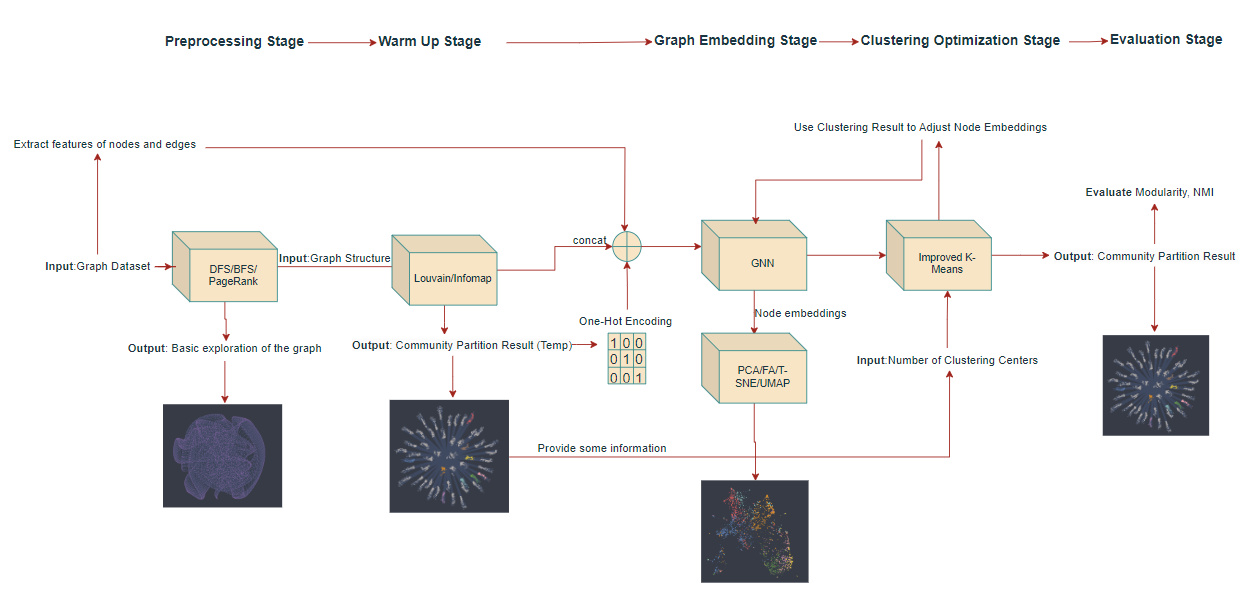
\includegraphics[width=1.0\textwidth]{Figure_3.png} % Adjust the width to scale the image
    \caption{Our Model Architecture}
    \label{fig: Our Model Architecture}
\end{figure}
\section{Stage One: Preprocessing Stage}
Many scholars overlook graphs' preprocessing and essential exploration, but different graphs have different topological structures. This also means they have different connectivity, degree distribution, and degree-degree correlation~\cite{borner2007network}. So before conducting graph community detection, we need to preprocess the graph.

In our model, connectivity is critical for evaluating preliminary communities, as different connectivity components necessarily belong to other communities. We use DFS to count the number of connected components in the graph data. Then, we use each connected component as the initial community partition.
\section{Stage Two: Warm-Up Stage}
Before formally training the model, we introduced a Warm-Up Stage. We use Louvain to partition the graph data into communities. Next, we use the results of community partitioning to assign one-hot representations to each node. The size of the hot encoding vector is the number of communities divided.

The Warm-Up stage helps machine learning models extract features, similar to pre-training. However, traditional pre-training requires initial training on large-scale data to enable the model to learn universal features or knowledge. Our method only needs to introduce the results of conventional community detection algorithms to help machine learning models reduce training time and improve model capabilities.
\section{Stage Three: Graph Embedding Stage}
The graph embedding stage is necessary to detect the graph community using machine learning methods. Section 2.4 of Chapter 2 introduces the graph embedding methods of different machine learning models. The basic idea of the graph embedding stage can be summarised using Formula 3.1.
\begin{equation}
h_v^{(k)} = \text{Update}\left(h_v^{(k-1)}, \text{Aggregate}\left(\{h_u^{(k-1)} \mid u \in \mathcal{N}(v)\}\right)\right)
\label{eq: Graph Embedding Stage}
\end{equation}
That is, features from the node's previous layer and its neighbouring features are aggregated to update the node's new features.
\section{Stage Four: Clustering Optimization Stage}
After obtaining the graph embedding vector, we put the graph embedding into the k-means clustering function for iteration and clustering. Finally, we use the output allocation matrix and modularity for loss calculation. According to Bryan Wilder et al.'s research~\cite{wilder2019end}, we can use modularity as the optimisation objective function. Our clustering optimisation process is summarised in Figure 3.2.
\begin{figure}[h!] % 'h!' attempts to position the figure here
    \centering
    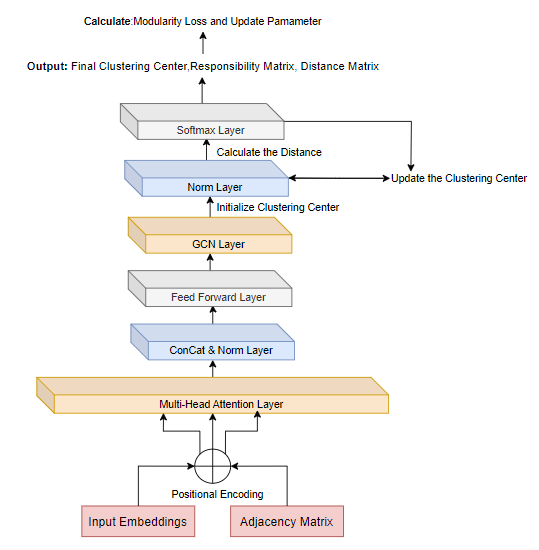
\includegraphics[width=0.8\textwidth]{Figure_4.png} % Adjust the width to scale the image
    \caption{Clustering Optimization Process}
    \label{fig: Clustering optimisation process}
\end{figure}
Calculating the responsibility matrix is shown in Formula 3.2, the calculation of the modularity matrix is shown in Formula 3.3, and the calculation of modularity loss is shown in Formula 3.4.
\begin{equation}
r_{ij} = \frac{\exp(-\text{temp} \cdot d_{ij})}{\sum_{l=1}^K \exp(-\text{temp} \cdot d_{il})}
\label{eq: Responsibility}
\end{equation}
Where:
\begin{itemize}
    \item temp is a temperature parameter.
    \item $d_{ij}$ represents the distance from data point $x_{i}$ to cluster center $y_{j}$
\end{itemize}
\begin{equation}
\text{Mod} = A - \frac{\text{Deg} \cdot \text{Deg}^T}{\sum_{i,j} A_{ij}}
\label{eq: Mod}
\end{equation}
Where:
\begin{itemize}
    \item Mod is used to evaluate the quality of community segmentation in graphs.
    \item A is the adjacency matrix.
    \item Deg is the degree matrix.
\end{itemize}
\begin{equation}
\text{Loss} = \frac{1}{\sum_{i,j} \text{bin\_adj}_{ij}} \cdot \text{Tr}(r^T \cdot \text{Mod} \cdot r)
\label{eq: Loss}
\end{equation}
Where:
\begin{itemize}
    \item $bin\_adj_{ij}$ is the binary adjacency matrix.
    \item r is the responsibility matrix.
    \item $Tr(*)$ is the trace of the matrix.
\end{itemize}
After we have the expression of the loss function, we can update the parameters through backpropagation using the chain rule(Formula 3.5).
\begin{equation}
\frac{\partial \text{Loss}}{\partial \theta} = \frac{\partial \text{Loss}}{\partial r} \cdot \frac{\partial r}{\partial \theta}
\label{eq: chain rule}
\end{equation}
The strategy of the clustering optimisation stage can be changed by changing the loss function. For example, binary cross entropy loss can be optimised for link prediction~\cite{kumar2020link}. This article aims to improve the effectiveness of community detection, so the loss function of Formula 3.4 is used.
\section{Stage Five: Evaluation Stage}
The evaluation stage is the final step in model design, where we use the \textbf{modularity} of community partitioning as the primary evaluation metric and \textbf{visualise the community} for further research. In the design phase, the specific implementation of modularity is shown in Formula 3.6. Unlike Formula 2.3, it refines the implementation of the indicator function.
\begin{equation}
Q = \frac{1}{2m} \sum_{ij} \left[ A_{ij} - \frac{k_i k_j}{2m} \right] r_{uk}\cdotr_{vk}
\label{eq:modularity2}
\end{equation}
This is also the method most scholars~\cite{wu2020deep}~\cite{agrawal2020community} to evaluate graph community detection models. However, the novelty of our design lies in assessing the Normalized Mutual Information(NMI)~\cite{zhang2015evaluating} of community segmentation results and accurate labels on annotated data. The calculation of NMI is shown in Formulas 3.7, 3.8, and 3.9.
\begin{equation}
I(U; V) = \sum_{u \in U} \sum_{v \in V} p(u, v) \log \frac{p(u, v)}{p(u)p(v)}
\label{eq: I(U,V)}
\end{equation}

\begin{equation}
H(U) = - \sum_{u \in U} p(u) \log p(u)
\label{eq:H(U)}
\end{equation}
\begin{equation}
\text{NMI}(U, V) = \frac{I(U; V)}{\sqrt{H(U) H(V)}}
\label{eq: NMI(U,V)}
\end{equation}
Where:
\begin{itemize}
    \item $I(U; V)$ is the mutual information between two random variables, U and V.
    \item $H(U)$ is the entropy of the random variable U.
    \item $p(u, v)$ is the joint probability distribution of U and V.
    \item $p(u)$ is the marginal probability distribution of U.
    \item $p(v)$ is the marginal probability distribution of V.
\end{itemize}
We can measure the correlation between clustering results and accurate labels through NMI. If the NMI of our community detection results is high, we can use community detection algorithms to annotate unlabeled data.
\chapter{Implementation}
\label{chap:Implementation}
Chapter 4 introduces the model's implementation details and data preparation. Section 4.1 introduces the experimental environment and the external packages that must be installed. Then, in section 4.2, we introduce the experiment's hardware environment and computing resources. In section 4.3, we introduce the preparation of data. We focus on exploring Telecom Graph data and visualising some Telecom Graph data. At the same time, to ensure the experiment's rigour, we introduce other different datasets and calculate the PageRank values of all datasets. The preprocessing stage of the model is also reflected in Chapter 4. Finally, we introduce the selection range of model layers.
\section{Experimental Environment}
For this data science project, we use Python 3.9 as the programming language, Jupter Notebook~\cite{kluyver2016jupyter} as the computing environment, and Ubuntu 18.04 as the image. At the same time, we synchronously upload the work process, program source code, and experimental results to GitHub during our work. The packages with compatible versions we need to install on Python are shown in Table 4.1.
\begin{table}[!htbp] 
\centering 
\label{External Packages} 
\caption{External Packages} 
\vspace{5pt} 
\begin{tabular}{cccc} 
\hline 
Package &Version&Package&Version \\ 
\hline
torch-geometric &2.3.1&torch&1.13.1 \\
torchaudio &0.13.1&torchvision&0.14.1 \\
python-louvain &0.16&networkx&2.8.8 \\
sklearn &1.5.1&infomap&2.8.0 \\
matplotlib &3.9.0&numpy&1.16.4 \\
pandas & 2.2.2&scipy&1.13.1\\
\hline
\end{tabular}
\end{table}

All external packages are essential for running experiments. Before replacing the experimental environment to reproduce the code, it is necessary to check whether the external package is installed and the version is compatible.

\section{Computation Resources}
All experiments were conducted on Huawei Cloud's ModelArts Platform~\cite{hu2021optimal}. Due to the time-consuming nature of community detection for large-scale graphs, we need to use cloud computing technology instead of running our computers for a day and a night. At the same time, to save certain costs, we also use a local computer for small-scale graph experiments and code debugging. The specific resources we use are shown in Table 4.2.
\begin{table}[!htbp] 
\centering 
\label{Computation Resources} 
\caption{Computation Resources} 
\vspace{5pt} 
\begin{tabular}{cc} 
\hline 
Resource &Specification \\ 
\hline
CPU(Cloud) &Intel 8vCPUs 32GB \\
GPU(Cloud) &Tnt 004 16GB \\
Disk(Cloud) &EVS 1024GB \\
CPU(Local) &Intel i7-10875H 8GB\\
GPU(Local) &GeForce GTX 1650 4GB \\
\hline
\end{tabular}
\end{table}
\section{Dataset Description}
The Telecom Graph we use is provided by Stanford Network Analysis Platform(SNAP)~\cite{snapnets}. The basic information of the Telecom Graph is shown in Table 4.3.
\begin{table}[!htbp] 
\centering 
\label{Basic Infomation} 
\caption{Basic Infomation of the Telecom Graph} 
\vspace{5pt} 
\begin{tabular}{cc} 
\hline 
Node Information &Edge Information \\ 
\hline
User: 300 Features &User-Buy-Package: 2 Features \\
Package: 138 Features &User-Use-App: 111 Features \\
App: 41 Features & User-Live-Cell: 37 Features \\
Cell: 1000 Features &\\
\hline
\end{tabular}
\end{table}
In the preprocessing stage, the dataset has 20 connected components of the same size. And every connected component graph is isomorphic. The statistics for a connected component are shown in Table 4.4.
\begin{table}[!htbp] 
\centering 
\label{Basic Infomation} 
\caption{Statistics for one Connected Component} 
\vspace{5pt} 
\begin{tabular}{ccccc} 
\hline 
Node &User&Package&App&Cell \\ 
\hline
Count&5000&19&50&3450\\
\hline
\end{tabular}
\end{table}

In Telecom Graph data, if two subgraphs are connected components, they do not have any shared cells, programs, or packages. For example, the North American and Asian branches of the same operator may generate two connected components. As shown in Figure 4.1, we create a virtual map to display the different connected components.
\begin{figure}[h!] % 'h!' attempts to position the figure here
    \centering
    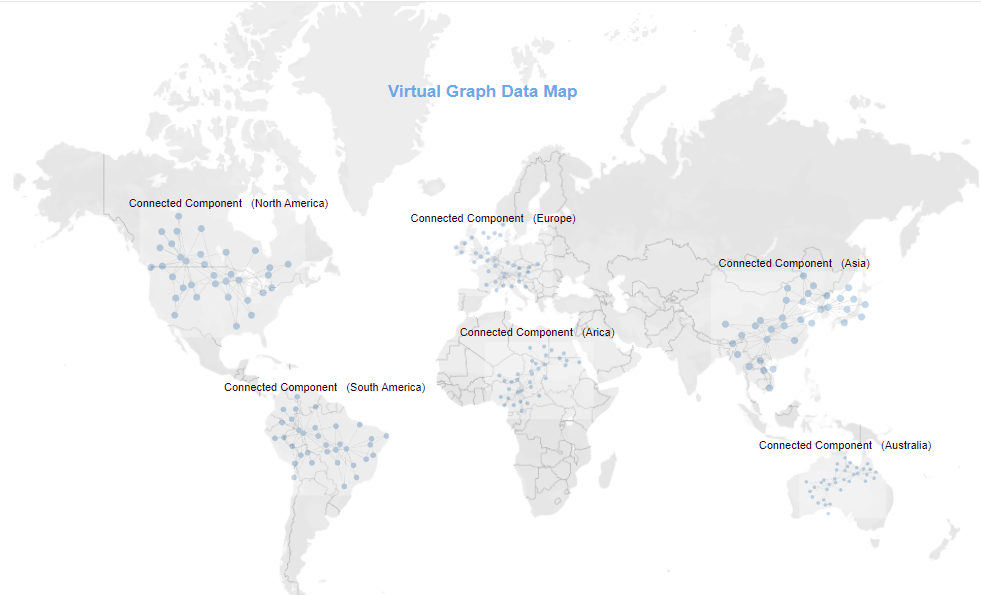
\includegraphics[width=1.0\textwidth]{Figure_5.png} % Adjust the width to scale the image
    \caption{Virtual Graph Data Map}
    \label{virtual Graph Data Map}
\end{figure}

If 20 connected components are directly used as the detected communities, the modularity of community partitioning reaches 0.9499. Although this division is mathematically perfect, it does not bring any innovative discoveries to operators. It is difficult to provide personalised services for users in single connected component areas, and it is also difficult to divide base stations reasonably. In short, dividing the community too large is not beneficial because it is challenging to provide commercial value. Then, we visualise a single connected component, as shown in Figure 4.2.
\begin{figure}[h!] % 'h!' attempts to position the figure here
    \centering
    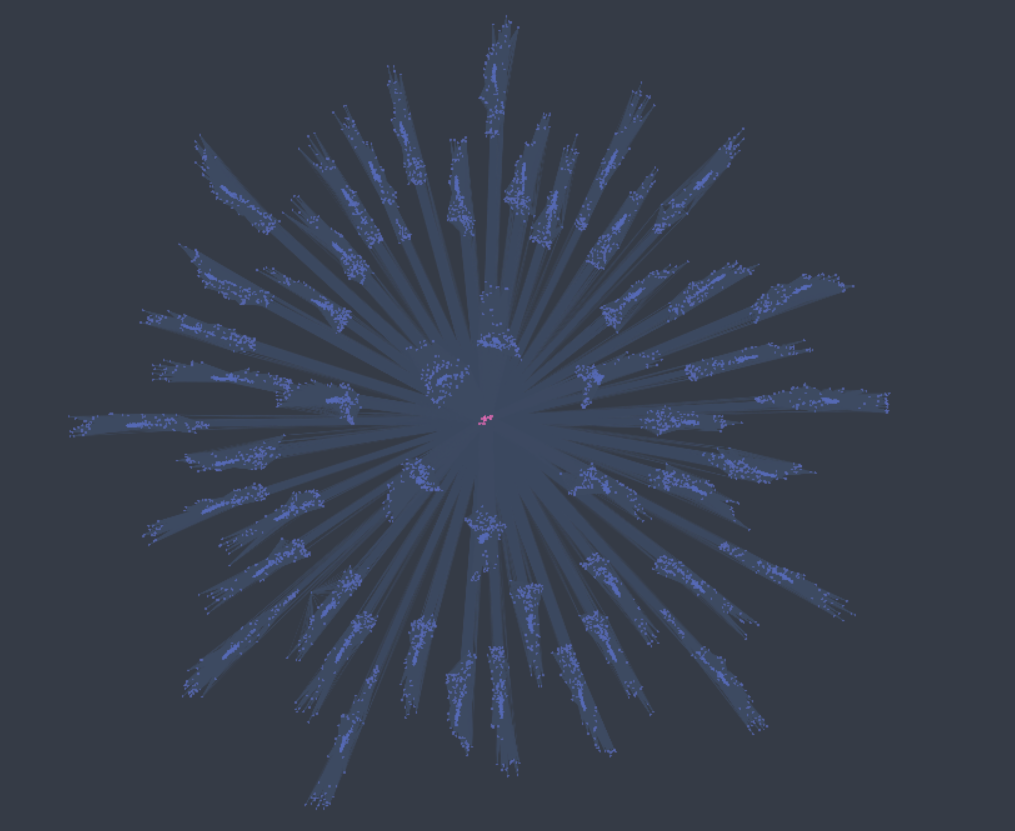
\includegraphics[width=1.0\textwidth]{Figure_6.png} % Adjust the width to scale the image
    \caption{Display of a Single Connected Component}
    \label{virtual Graph Data Map}
\end{figure}
From Figure 4.2, we can see that there are also many apparent clusters in a single connected component. After detecting each small cluster of connected components separately, we merge the results of all connected components into a complete community detection result, which is more commercially valuable.

We also used other types of datasets to demonstrate the superiority of our model, especially supervised datasets such as the paper citation dataset Cora~\cite{mccallum2000automating}, Citeseer~\cite{giles1998citeseer}, Pubmed~\cite{canese2013pubmed}; Protein structure dataset: Protein~\cite{jha2022prediction}; Social network dataset: Actor~\cite{caniels2008actor}. Their statistical information is shown in Table 4.5.
\begin{table}[!htbp] 
\centering 
\label{Basic Infomation} 
\caption{Statistics of the Datasets used in the Article} 
\vspace{5pt} 
\begin{tabular}{ccccccc} 
\hline 
Dataset &Node&Edge&Density&Connected Component&Mean Degree&Label \\ 
\hline
Telecom (Entire)&170380&8900000&0.0006&20&104.47&Null \\
Telecom (Sub)&8519&445000&0.0122&1&104.47&Null\\
Cora&2708&5278&0.0014&78&3.89&2708\\
Pubmed&19717&44324& 0.0002&1&4.49&19717\\
Citeseer&3327&4552&0.0008&438&2.73&3327\\
Protein&27&46&0.1310&1&3.41&Null\\
Actor&7600&26752&0.0009&1&7.04&7600\\
\hline
\end{tabular}
\end{table}
From Table 4.5, it can be seen that the size and properties of the datasets we used vary greatly, which can greatly improve the rigour of the model. Next, we use the PageRank algorithm~\cite{page1999pagerank} to calculate the nodes of all datasets, as shown in Figure 4.3.
\begin{figure}[h] % 'h!' attempts to position the figure here
    \centering
    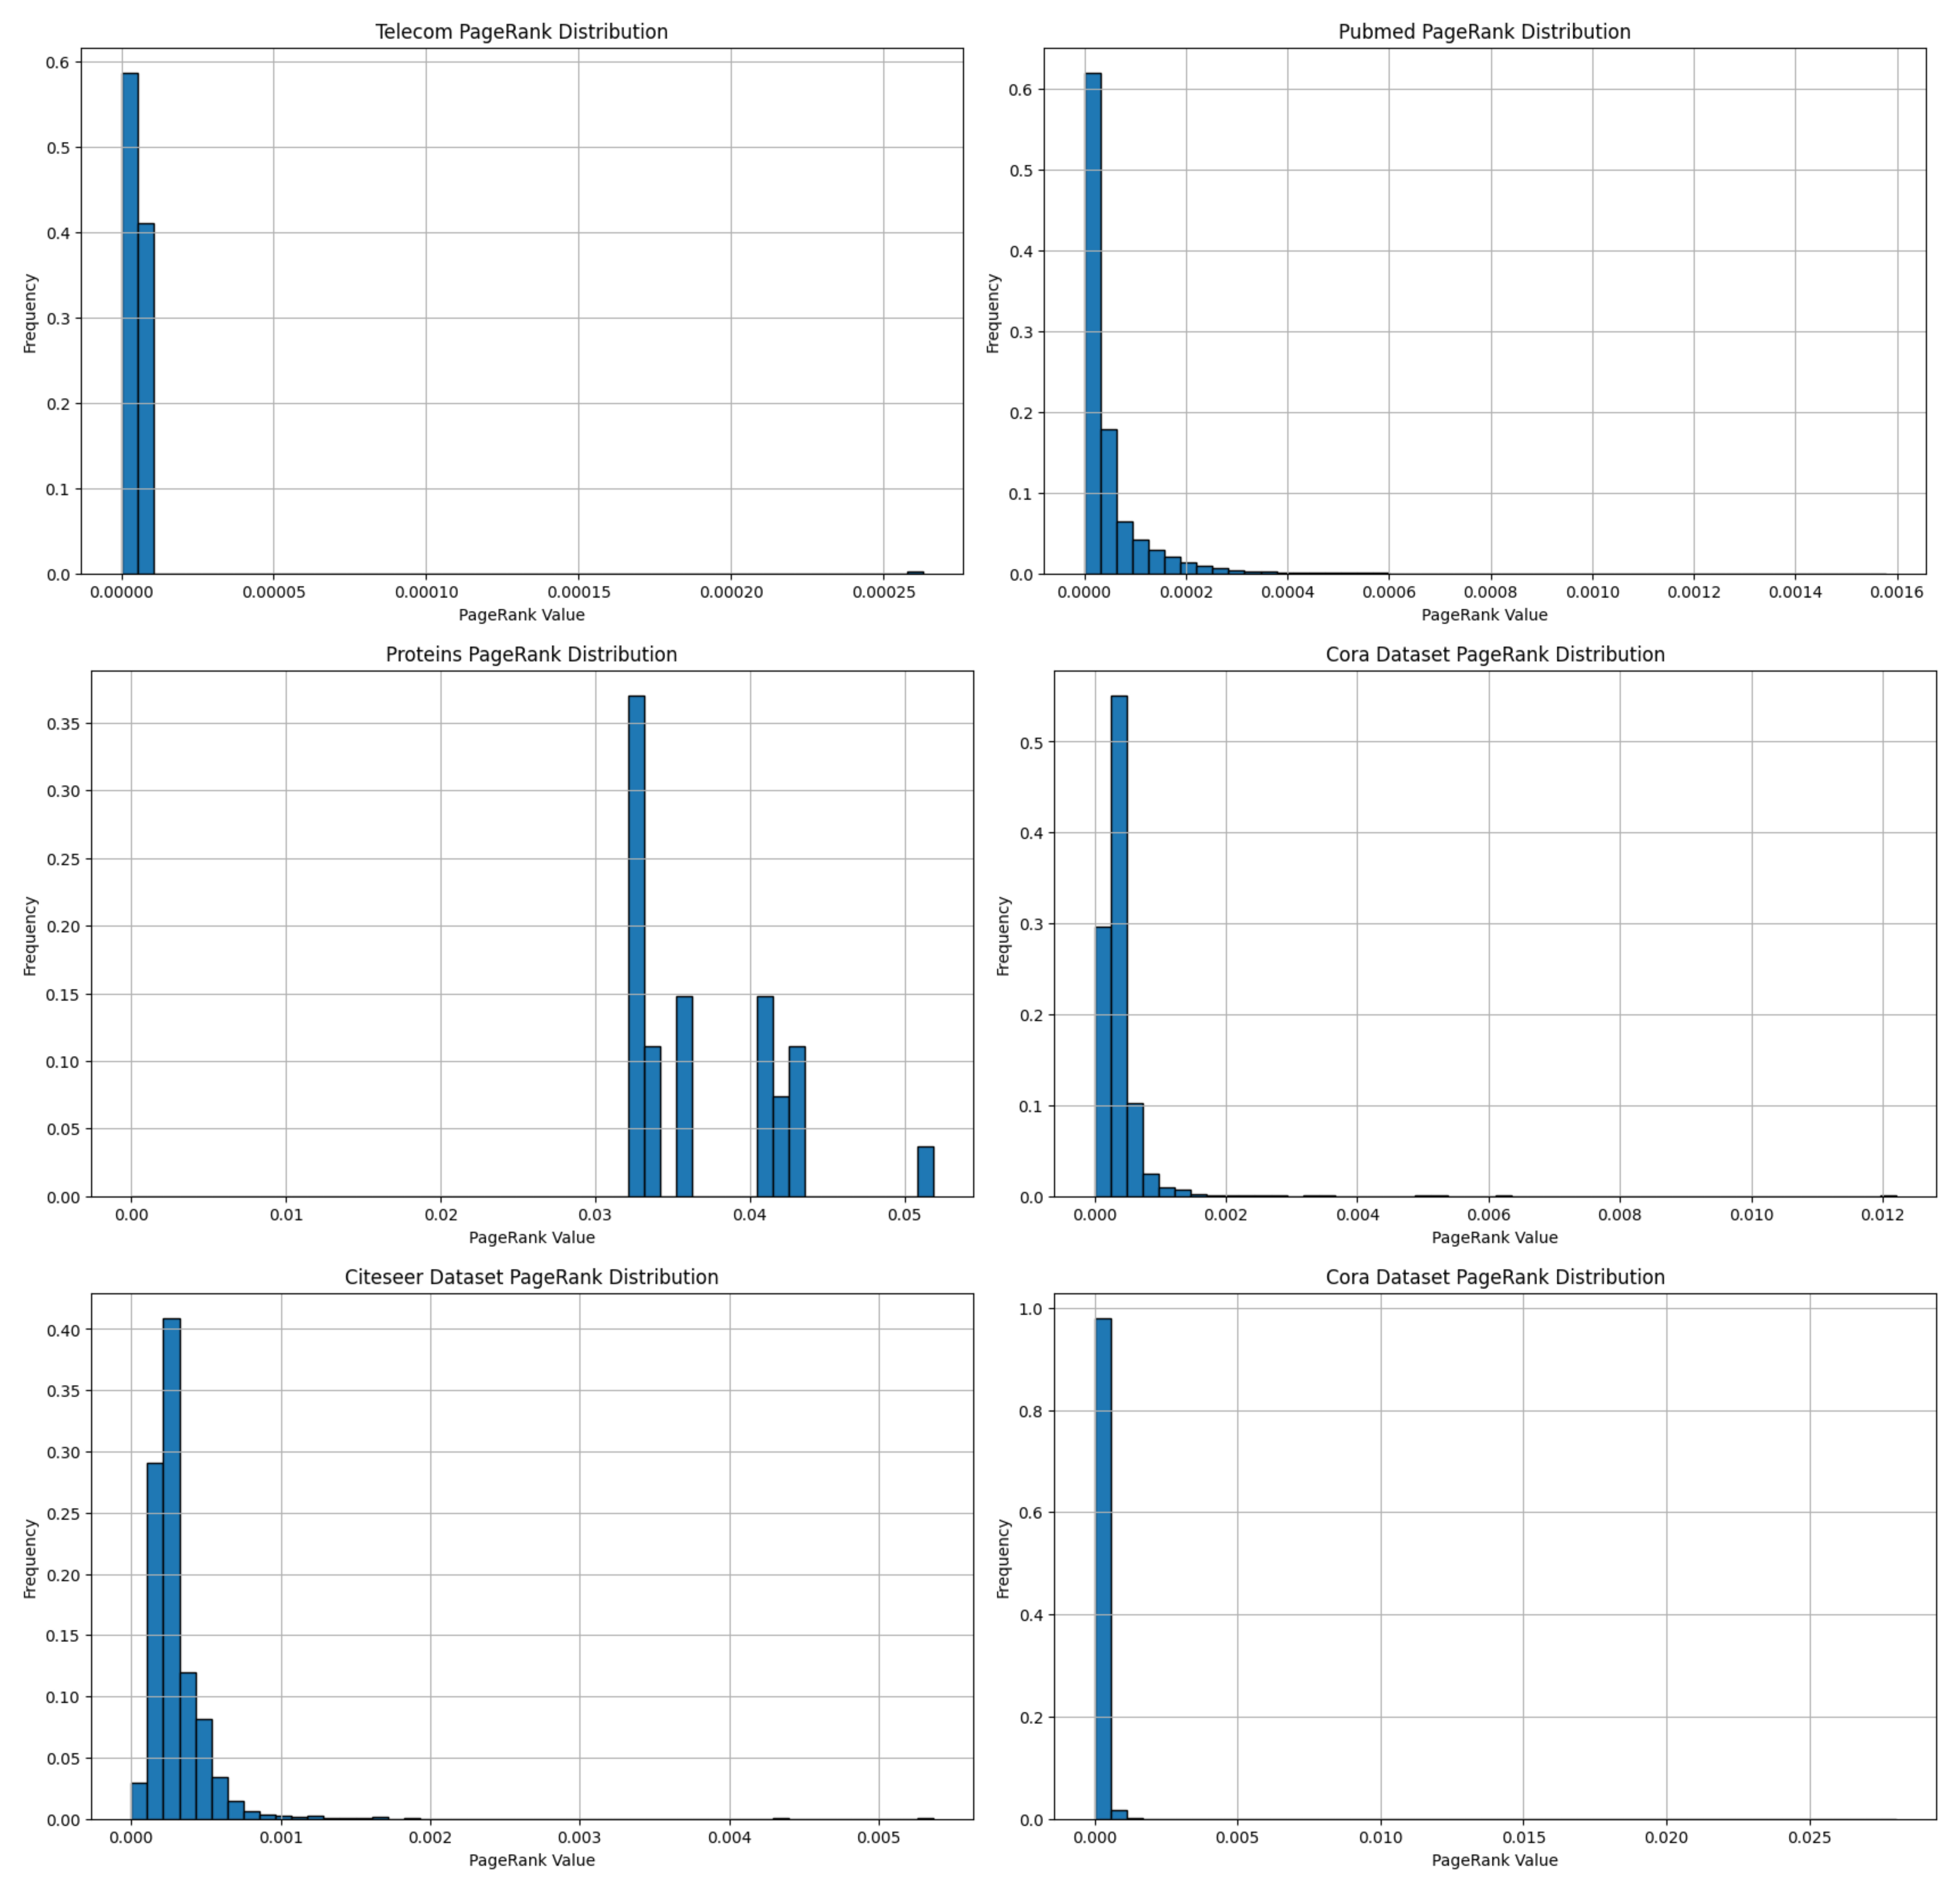
\includegraphics[width=0.8\textwidth]{Figure_8.png} % Adjust the width to scale the image
    \caption{PageRank Distribution}
    \label{virtual Graph Data Map}
\end{figure}
We need to focus on nodes with high PageRank. In the telecom graph, the package node has the highest PageRank value; in the paper citation network, papers with high citation counts have the highest PageRank values; and in protein and social networks, individuals with frequent interactions have the highest PageRank values. Nodes with high PageRank values play an essential role in building communities.
\section{Model Layers}
In Graph Machine Learning tasks, the design of model layers is crucial. To prevent the problem of \textbf{Over Smoothing}, our model layer design is based on other scholars' articles, as shown in Table 4.6.
\begin{table}[!htbp] 
\centering 
\label{Basic Infomation} 
\caption{Model Layers} 
\vspace{5pt} 
\begin{tabular}{ccc} 
\hline 
Layer &Algorithm&Hidden Size Range \\ 
\hline
Layer 1&GNN&[50, 200]\\
Layer 2&GNN&[50, 200]\\
Layer 3 (Optional)&GNN&[50, 150]\\
Layer 4 (Optional)&GNN&[50, 100]\\
Layer 5 (Optional)&GNN&[50, 100]\\
Layer 6&K-Means Cluster&Null\\
Layer 7&K-Means Cluster&Null\\
\hline
\end{tabular}
\end{table}
The selection of model hyperparameters and layers must be validated based on experimental results for different datasets. Chapter 5 provides further optimisation and evaluation.




% -----------------------------------------------------------------------------

\chapter{Critical Evaluation}
\label{chap:evaluation}
In Chapter 5, we introduce the evaluation process of our model. Section 5.1 introduces the model's hyperparameter selection and training process. By comparing the effects of different hyperparameters on the model training process, we selected the hyperparameters that achieve the best performance of the model. In Section 5.2, we comprehensively evaluate the performance of our model and compare the performance differences between different models. In Section 5.3, we conduct a case study on the detected communities and extract the commercial value of the community detection results for BT. In Section 5.4, we conduct ablation experiments to demonstrate the rigour of our model.
\section{Hyperparameters Selection and Model Training}
The selection of hyperparameters is crucial in improving the model's performance. Moreover, hyperparameters cannot be learned by the loss function, and their selection depends on the specific dataset and task. We must conduct tests and evaluations to determine the best set of hyperparameters. The search space for hyperparameters is shown in Table 5.1.
\begin{table}[!htbp] 
\centering 
\label{Basic Infomation} 
\caption{The Search Space for Hyperparameters} 
\vspace{5pt} 
\begin{tabular}{cc} 
\hline 
Parameter &Value Range \\ 
\hline
Learning Rate& [5e-5,0.05]\\
Weight Decay&[5e-5, 0.01]\\
Cluster Temperature&[20,200]\\
Clustering Iterations&[1,5]\\
\hline
\end{tabular}
\end{table}
For each dataset, we need to re-experiment to determine the optimal hyperparameters. Due to space limitations, we demonstrate the training process of different hyperparameters on the Telecom dataset, as shown in Figure 5.1.
\begin{figure}[h] % 'h!' attempts to position the figure here
    \centering
    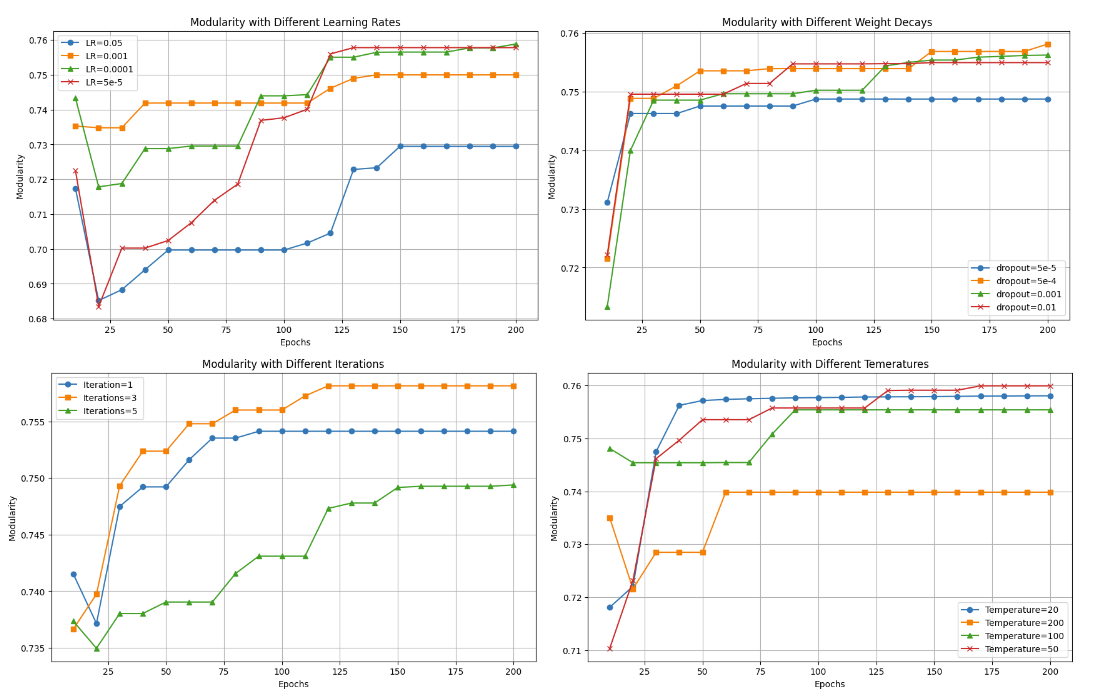
\includegraphics[width=0.8\textwidth]{Figure_9.png} % Adjust the width to scale the image
    \caption{LEGC (GCN) Training Process of Different Hyperparameters}
    \label{virtual Graph Data Map}
\end{figure}
From Figure 5.1, we can conclude that hyperparameters significantly impact model training. An excessively high learning rate can trap the model in local optima, while a low weight decay can lead to overfitting. An appropriate number of clustering iterations and temperature can improve model performance. 

Also, We can note that the values of the first epoch are not the same, and the difference is significant. This is due to the random initialisation of cluster centres, as different random cluster centres will have different starting modularity. However, we cannot specify the cluster centre, as the cluster centres of different datasets need to be updated iteratively. So, we need to conduct multiple experiments under the same hyperparameter settings to determine the optimal hyperparameter combination. 

Finally, we obtained the optimal hyperparameter sets after numerous experiments, as shown in Table 5.2.
\begin{table}[!htbp] 
\centering 
\label{Basic Infomation} 
\caption{The Optimal Hyperparameter Sets} 
\vspace{5pt} 
\begin{tabular}{ccccc} 
\hline 
Dataset &Learning Rate&Weight Decay&Cluster Temperature&Clustering Iterations \\ 
\hline
Telecom& 0.0001&5e-4&50&3\\
Cora& 5e-5&0.001&30&1\\
Pubmed& 5e-5&5e-4&30&1\\
Citeseer& 0.0001&0.001&20&5\\
Protein& 0.001&5e-5&60&1\\
Actor& 5e-4&5e-5&50&5\\
\hline
\end{tabular}
\end{table}
Table 5.2 concludes that the optimal hyperparameter selection varies for different datasets. For small datasets such as Protein, we can use higher learning rates to accelerate the training process, while for large datasets, high learning rates and low weight decay can significantly affect the model's performance.

Next, we use different GNN models to train our datasets. During the training process after changing the GNN model, we also need to fine-tune the hyperparameters to achieve the optimal model. Our training process is shown in Figure 5.2.
\begin{figure}[h!] % 'h!' attempts to position the figure here
    \centering
    \includegraphics[width=1.0\textwidth]{Figure_10.png} % Adjust the width to scale the image
    \caption{LEGC Training Process of Different Datasets}
    \label{virtual Graph Data Map}
\end{figure}
From Figure 5.2, we can conclude that our different GNN models have successfully converged on various datasets. For the small graph dataset Protein, each GNN model achieves optimal performance and does not change after 100 to 200 epochs. In contrast, there is some fluctuation in the first 1000 epochs for large graph datasets, usually reaching optimal performance and no change after 1500 epochs. Moreover, different GNN models perform differently on various datasets, and not the most complex algorithm (GT) necessarily performs the best on the dataset. We must flexibly adjust the graph embedding algorithm for different datasets to achieve optimal performance. Next, we will discuss the model's various performance indicators.
\section{Performance of Different Models on Datasets}
Based on our trained model, we can obtain various machine learning models' performance (modularity) on different datasets, as shown in Table 5.3.
\begin{table}[!htbp] 
\centering 
\label{Basic Infomation} 
\caption{Modularity of LEGC(Different GNNs) on Datasets} 
\vspace{5pt} 
\begin{tabular}{ccccccc} 
\hline 
Models &Telecom&Cora&Pubmed&Citeseer&Protein&Actor \\ 
\hline
LEGC(GCN)&\textbf{0.7605}&0.7533&\textbf{0.6200}&0.7724&0.6618&0.4614\\
LEGC(GraphSAGE)&0.7586&0.7535& 0.5653&0.7718&0.6618&0.4594\\
LEGC(GAT)&0.7604&0.7437&0.5936&\textbf{0.7781}&0.6618&0.4509\\
LEGC(GT)&0.7572&\textbf{0.7563}&0.5830&0.7765&0.6618&\textbf{0.4890}\\
\hline
Best Result&0.7605&0.7563&0.6200&0.7781&0.6618&0.4890\\
\hline
\end{tabular}
\end{table}
At the same time, we calculate the time for each model to converge to its optimal performance, as shown in Figure 5.3.
\begin{figure}[h!] % 'h!' attempts to position the figure here
    \centering
    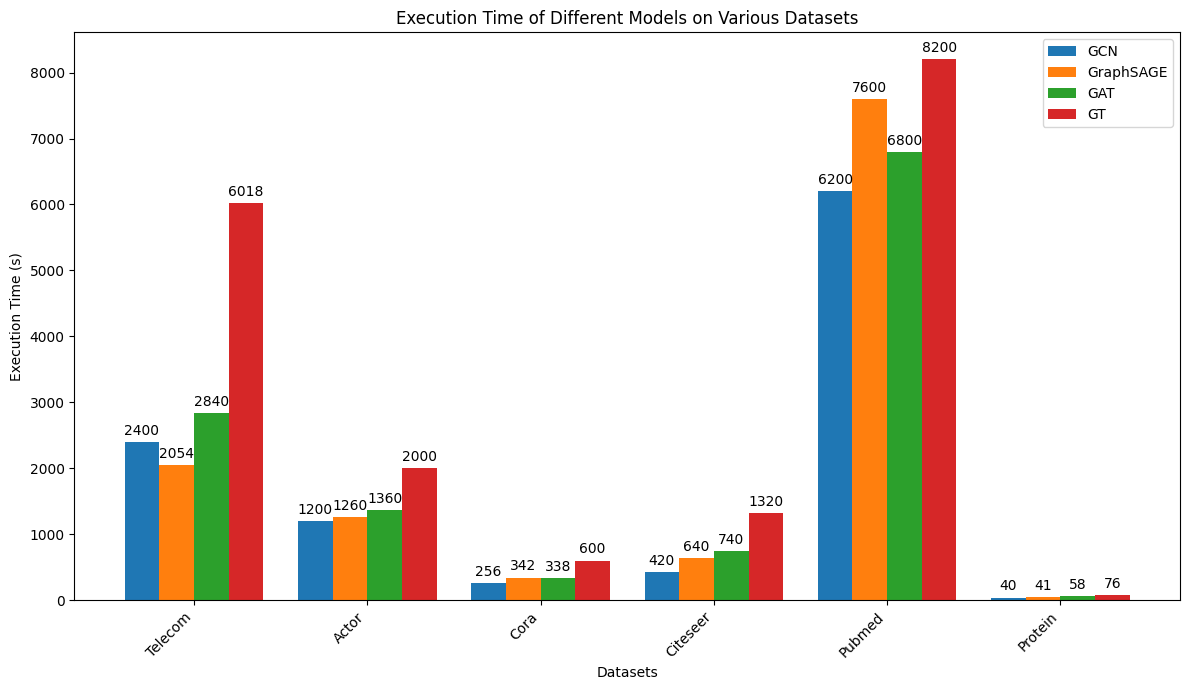
\includegraphics[width=0.9\textwidth]{Figure_11.png} % Adjust the width to scale the image
    \caption{Execution Time of LEGC(Different GNNs) on Various Datasets}
    \label{virtual Graph Data Map}
\end{figure}
From Figure 5.3 and Table 5.3, we can conclude that different models have different training times, with the most complex GT model taking the longest time, while GCN and GraphSAGE models taking the shortest time. When we choose the final model, we can choose the model with the best performance. However, when selecting models with the same performance or little difference in performance, we can choose simpler models to reduce training time. 

Based on the comprehensive execution time and performance, the graph embedding models we selected for different datasets are shown in Table 5.4. Our subsequent evaluation results will focus on the best GNN embedding model to save the article's length and reduce unnecessary discussions.
\begin{table}[!htbp] 
\centering 
\label{Basic Infomation} 
\caption{the Best GNN Embedding Model of LEGC} 
\vspace{5pt} 
\begin{tabular}{|cccccc|} 
\hline 
Telecom&Cora&Pubmed&Citeseer&Protein&Actor \\ 
\hline
GCN&GT&GCN&GAT&GCN&GT\\
\hline
\end{tabular}
\end{table}
Next, we use PCA to visualise the graph embedding results of each dataset, as shown in Figure 5.4. 
\begin{figure}[h!] % 'h!' attempts to position the figure here
    \centering
    \includegraphics[width=0.8\textwidth]{Figure_14.png} % Adjust the width to scale the image
    \caption{Visualization of Node Embeddings}
    \label{virtual Graph Data Map}
\end{figure}

At the same time, based on the trained graph embedding and community detection results, we calculated the average distance between the same class (same community) and the average distance between different classes (different communities) of the dataset. We calculated the NMI of the supervised dataset, as shown in Table 5.5.
\begin{table}[!htbp] 
\centering 
\label{Basic Infomation} 
\caption{Other Performance Metrics of the Datasets} 
\vspace{5pt} 
\begin{tabular}{ccccccc} 
\hline 
Metrics&Telecom&Cora&Pubmed&Citeseer&Protein&Actor \\ 
\hline
Average Same-Class Distance&0.6622&0.4221&0.0477&0.0591&0.3934&0.1267\\
Average Different-Class Distance&1.3605&1.2821&0.0899&0.1467&1.0782&0.4119\\
NMI&-&0.3955&0.1480&0.2061&-&0.0007\\
\hline
\end{tabular}
\end{table}

Figure 5.4 shows that nodes in the same community are well clustered into different clusters—the more communities we set up, the more clusters the graph embeds. Meanwhile, based on the values in Table 5.5, we can conclude that the results of our community detection have particular significance for annotated data. We can use community detection results to annotate unsupervised data, making it a supervised dataset for other scholars.



After demonstrating and discussing the performance of our model, we obtained the model performance of other scholars on the same dataset through CHUNAEV's review~\cite{chunaev2020community}, as shown in Table 5.6.
\begin{table}[!htbp] 
\centering 
\label{Basic Infomation} 
\caption{Performance Comparison of Different Models} 
\vspace{5pt} 
\begin{tabular}{cccc|cccc} 
\hline 
Datasets &Methods&Modularity & NMI&Datasets &Methods&Modularity & NMI\\ 
\hline
& LEGC&\textbf{0.756}&0.3955&& LEGC &\textbf{0.778}&0.2061\\
 &JWNMF~\cite{huang2017joint}&0.413&0.018&&JWNMF~\cite{huang2017joint}&0.321&0.007\\
 Cora &PCL-DC~\cite{yang2009combining}&0.697&\textbf{0.512}&Citeseer &PCL-DC~\cite{yang2009combining}&0.685&0.292\\
 & SCI~\cite{wang2016semantic}&-&0.178&& SCI~\cite{wang2016semantic}&-&0.092\\
 & PPSB-DC~\cite{chai2013combining}&-&0.466&&PPSB-DC~\cite{chai2013combining}&-&\textbf{0.387}\\
\hline
Protein & LEGC & \textbf{0.662}&-&Pubmed&LEGC &0.6200&0.1480\\
& GCN-CNM~\cite{wilder2019end}&0.180&-&&CPIP-PI~\cite{liu2015community}&-&\textbf{0.311}\\
\hline
Telecom & LEGC &0.761&-&Actor & LEGC & 0.489&0.0007\\
\hline
\end{tabular}
\end{table}
By comparing our model with other scholars' models, we find that our model performs the best in modularity among all methods. However, the performance of our supervised dataset's NMI is not optimal, and we believe this is due to our use of modularity to train the model, which tends to improve modularity rather than mutual information. If we use the mutual information of labels and clustering results from supervised datasets for training like other scholars, the mutual information of the model should be significantly improved.

\section{Case Study}
After discussing the performance of our model, we conduct a case study on Telecom Graph to provide a way for BT to use community detection results. Our Telecom Graph detection results are shown in Figure 5.5.
\begin{figure}[h] % 'h!' attempts to position the figure here
    \centering
    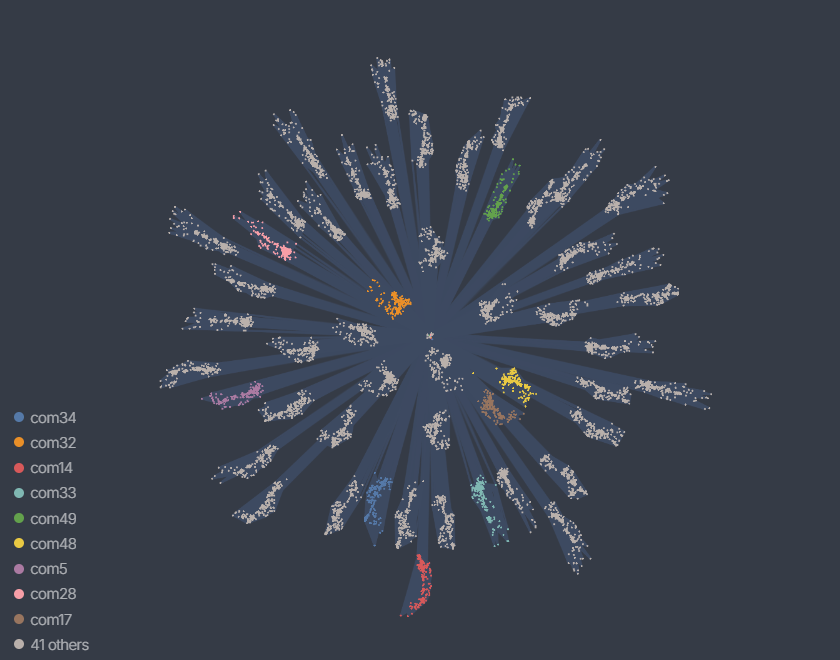
\includegraphics[width=1.0\textwidth]{Figure_12.png} % Adjust the width to scale the image
    \caption{Telecom Graph Detection Result}
    \label{virtual Graph Data Map}
\end{figure}
Figure 5.4 shows that the small clusters proposed in Chapter 4 have been successfully detected. This region's users, base stations, packages, and apps are divided into 50 small communities. We visualise some nodes of the same community, as shown in Figure 5.5. 
\begin{figure}[h] % 'h!' attempts to position the figure here
    \centering
    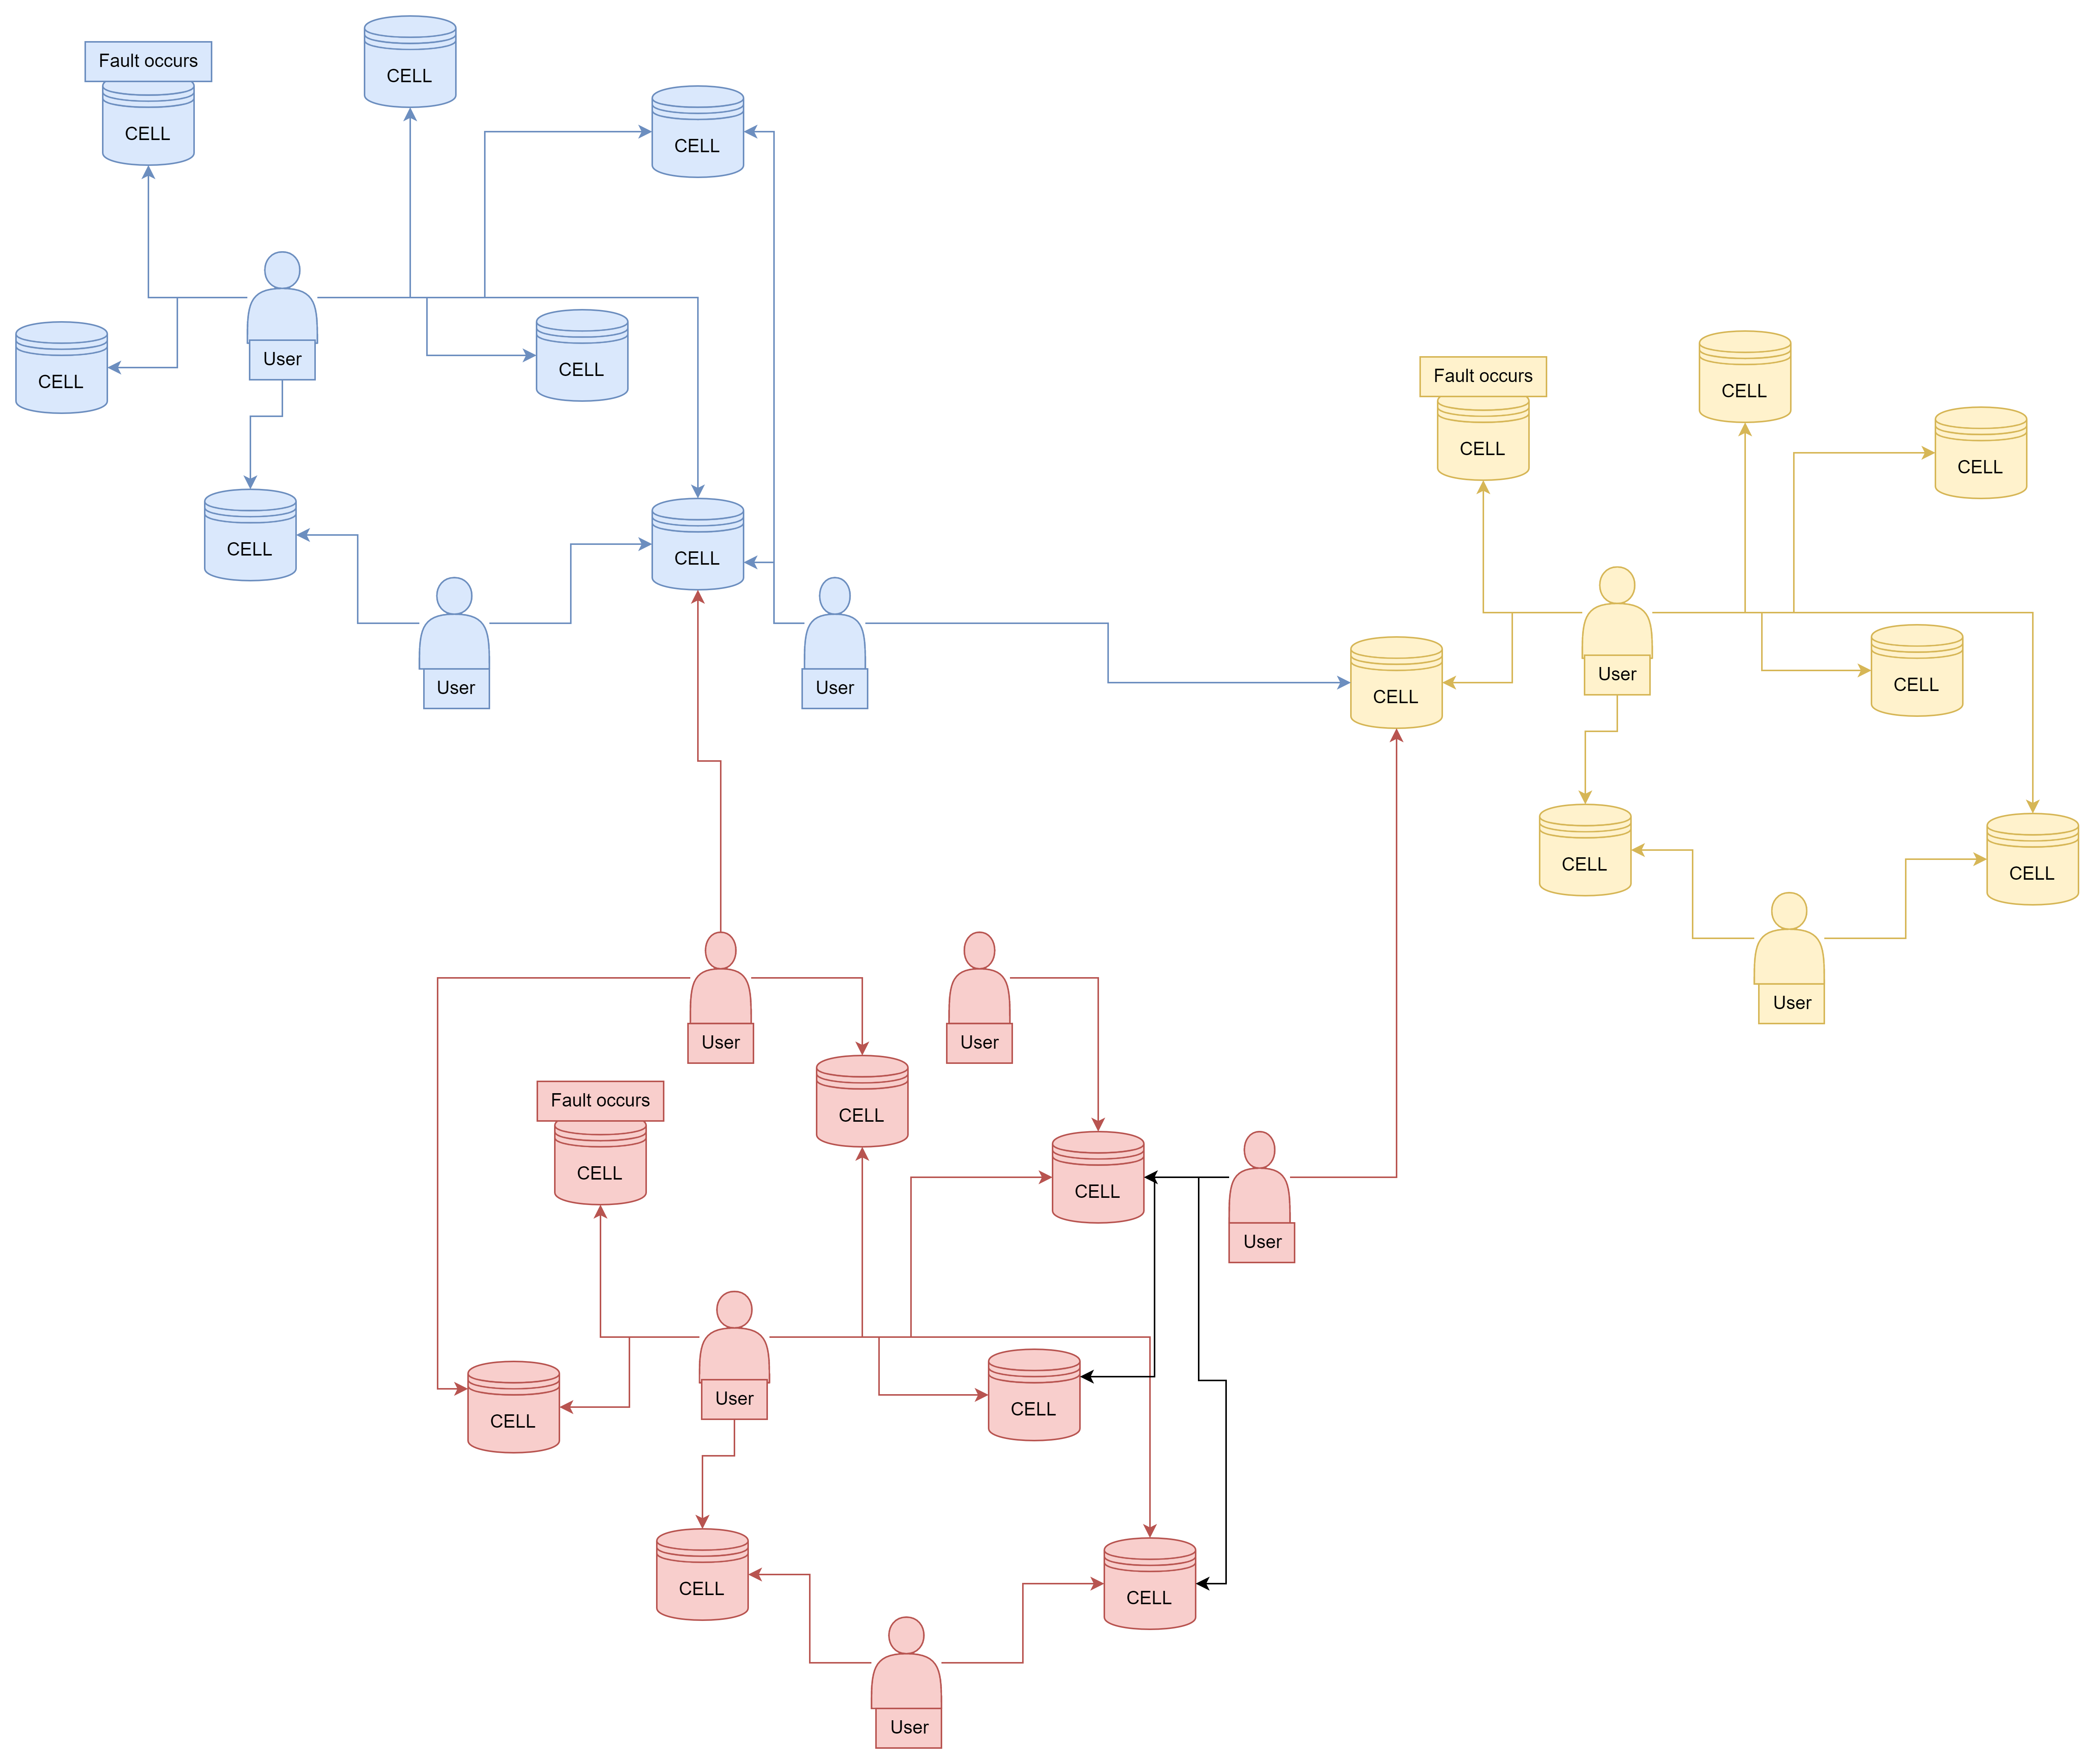
\includegraphics[width=0.8\textwidth]{Figure_13.png} % Adjust the width to scale the image
    \caption{User-Cell Communities}
    \label{virtual Graph Data Map}
\end{figure}
\begin{figure}[h] % 'h!' attempts to position the figure here
    \centering
    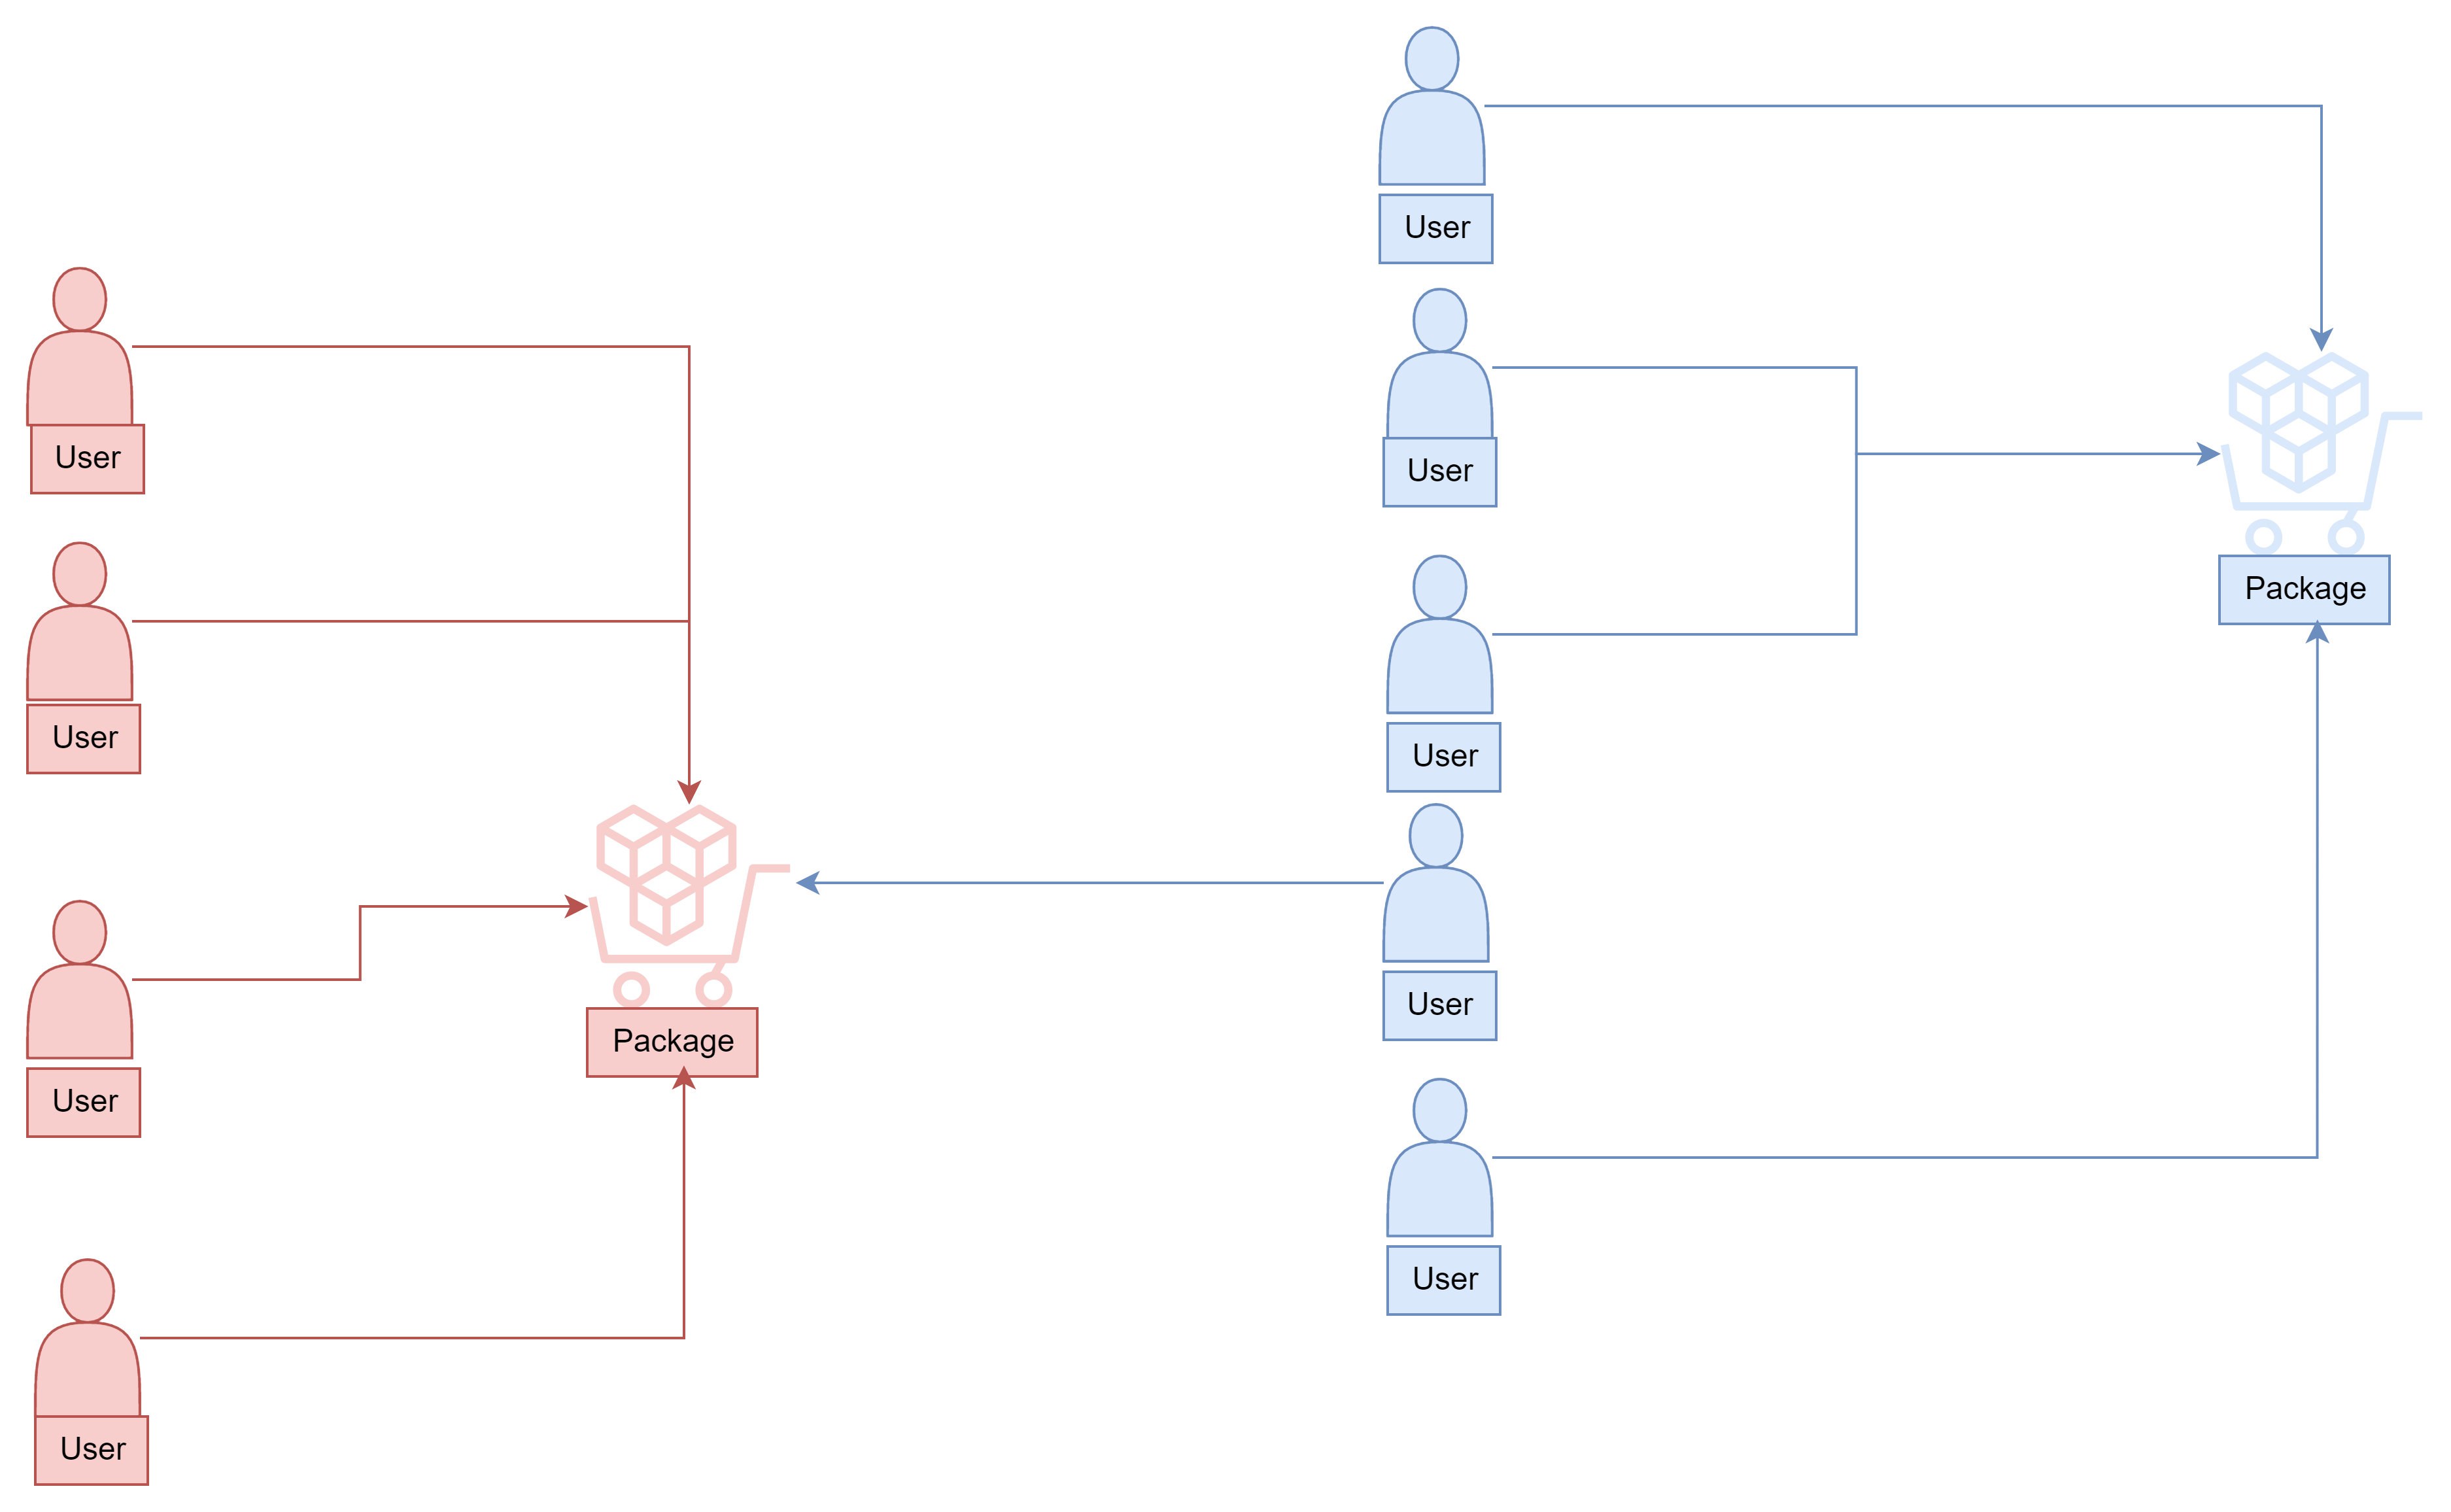
\includegraphics[width=0.8\textwidth]{Figure_19.png} % Adjust the width to scale the image
    \caption{User-Package Communities}
    \label{virtual Graph Data Map}
\end{figure}
Next, we will analyse how telecom operator BT should utilise this data.

\begin{itemize}
  \item \textbf{Case 1 Fault Detect}: As shown in Figure 5.6, When a user reports a network issue, BT can first search for the user's community, obtain all the cells in that community, and then investigate the problems of each base station one by one. Community testing can greatly help BT reduce retrieval costs.
  \item \textbf{Case 2 Network Environment Guarantee}: As shown in Figure 5.6, when a base station in a certain area stops working for various reasons (extreme weather, war, riots), BT needs to obtain other cells in the community where the base station is located and ensure their normal operation. This can greatly reduce the impact of the base station stopping working.
  \item \textbf{Case 3 Redundancy Planning}: Based on Case 1 and Case 2, we can derive the use of community detection for redundancy planning to avoid the problem of a single point of failure. Assuming a user's connected base station has a network problem, we must plan redundant lines in the same community and set up multiple communication paths to ensure network operation. Secondly, we must configure redundant devices for key network equipment (base stations, switches) in adjacent communities to ensure uninterrupted service in adjacent neighbourhoods. Thirdly, we must implement routing redundancy by designing routing redundancy within the same community. When a routing path fails, we can automatically convert it into an alternative route.  
  \item \textbf{Case 4 Personalized Application}: As shown in Figure 5.7, by detecting users and apps in the same community, we can obtain that the people in that community are loyal customers of the app. BT can use this data to study the app and users further, such as enhancing user stickiness through personalised updates and improvements or making users more frequent on the app through regular activities. Even if BT cannot access the relevant applications, it can still sell the community detection and analysis results to stakeholders.
  \item \textbf{Case 5 Micro Recommendation System}: Figure 5.7 shows we can build a community detection-based micro recommendation system. We can recommend a package launched by BT to users in the same community who have not yet purchased it because customers in the same community are likely to buy the same package. For example, we can treat Bristol customers as a community and recommend the 'Bristol Exclusive 20GB, National Universal 10GB' package to all Bristol customers.
\end{itemize}

\section{Ablation Experiment}
For experimental rigour, we need to conduct ablation experiments by removing components from our Chapter 3 design and observing whether the model performance has changed. If the model maintains the same performance after removing some elements, we can say that the component is redundant or useless. If eliminating some components significantly impacts the model's performance, that component is a practical design.
\subsection{Remove Warm-Up Stage}
The Warm-Up Stage is one of the article's most significant innovations, so we need to conduct focused ablation experiments to observe the model's performance changes after removing it. We selected the best model from Table 5.4 and followed the training process of the model's first 200 epochs before and after removal, as shown in Figure 5.8.
\begin{figure}[h] % 'h!' attempts to position the figure here
    \centering
    \includegraphics[width=0.8\textwidth]{Figure_15.png} % Adjust the width to scale the image
    \caption{Model Training Process Before and After Removing Warm Up}
    \label{virtual Graph Data Map}
\end{figure}
At the same time, we calculate the modularity changes of each dataset in the first epoch and the modularity changes after achieving optimal performance, as shown in Table 5.7.
\begin{table}[!htbp] 
\centering 
\label{Basic Infomation} 
\caption{Modularity Changes Before and After Removing Warm Up} 
\vspace{5pt} 
\begin{tabular}{cccc} 
\hline 
Datasets&Warm-Up Stage&Modularity (Epoch 1)&Modularity (Best)\\ 
\hline
Telecom&None&0.3312&0.7505\\
&Louvain&\textbf{0.7360}&\textbf{0.7605}\\

\hline
Cora&None&0.3511&0.7358\\
&Louvain&\textbf{0.4643}&\textbf{0.7563}\\
\hline
Citeseer&None&0.4521&0.7112\\
&Louvain&\textbf{0.5223}&\textbf{0.7724}\\
\hline
Actor&None&-0.0117& 0.4509\\
&Louvain&\textbf{0.0170}&\textbf{0.4890}\\
\hline
Protein&None&0.4113& 0.6618\\
&Louvain&\textbf{0.6418}&0.6618\\
\hline
Pubmed&None&0.4612& 0.6116\\
&Louvain&\textbf{0.4993}&\textbf{0.6200}\\
\hline
\end{tabular}
\end{table}
From Figure 5.8 and Table 5.7, we believe the Warm-Up Stage is a necessary step that significantly improves the training speed and model performance. It can accelerate long training times for large datasets, while for small datasets, it can enable the model to achieve optimal performance in the first ten epochs. 

We calculate that the modularity of the first Epoch increased by an average of 0.79, and the optimal modularity increased by an average of 0.037. However, the optimal performance has not been improved for small datasets, which we believe is because community detection in small datasets is relatively easy and can quickly converge to the best.


\subsection{Remove ClusterNet Stage}
Our model is based on the framework of Algorithm 1.3. We train and obtain the embedding model of nodes through ClusterNet. However, the methods of RandomWalk (Node2Vec) and Graph AutoEncoder can also get the embedding of nodes. Therefore, we must explore whether the model can achieve the same performance after removing ClusterNet and switching to other optimisation methods. We use Node2Vec and Graph AutoEncoder to calculate the node embedding vectors, then cluster them using K-means and calculate their modularity. The modularity of each model is shown in Figure 5.9.
\begin{figure}[h] % 'h!' attempts to position the figure here
    \centering
    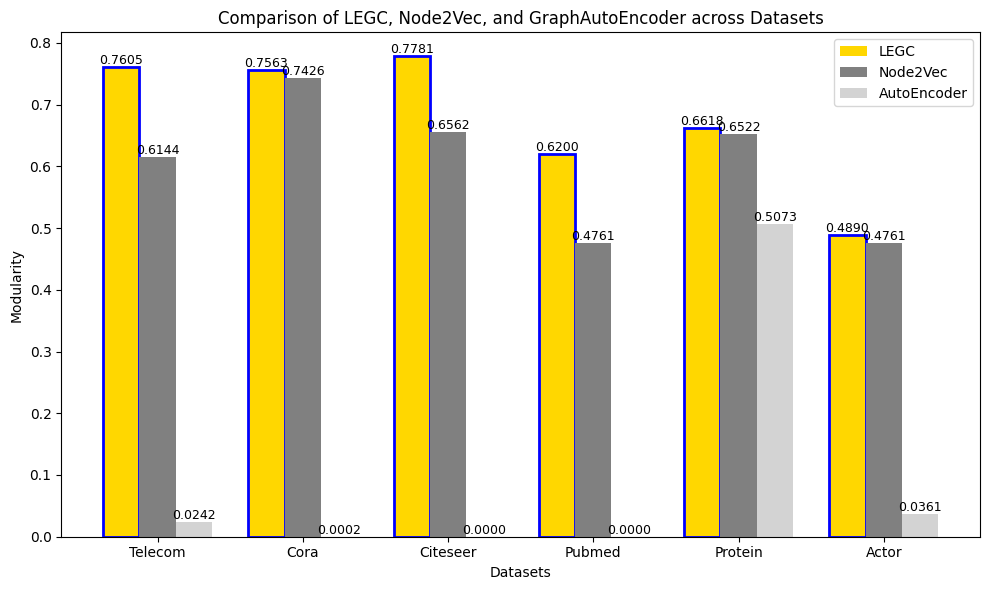
\includegraphics[width=0.9\textwidth]{Figure_16.png} % Adjust the width to scale the image
    \caption{Comparison of LEGC, Node2Vec, and GraphAutoEncoder across Datasets}
    \label{virtual Graph Data Map}
\end{figure}
From Figure 5.9, it can be concluded that optimising modularity using ClusterNet is necessary, and node embeddings trained on reconstruction errors using Graph AutoEncoder are more suitable for edge prediction tasks or node classification tasks (which many scholars have used in their articles~\cite{xie2021inductive}~\cite{guo2022multi}). The performance of Node2Vec in community detection is impressive, but it cannot repeatedly optimise graph embedding representations through loss functions. Therefore, we believe that Clusternet is necessary for maintaining model performance.
\subsection{Noise Environment Experiment}
Real data may contain noise, and obtaining a clean dataset is impossible. Therefore, we need to conduct experiments on this by adding some random noise to observe the performance changes of the model. Our noise strategy is shown in Table 5.8.
\begin{table}[!htbp] 
\centering 
\label{Basic Infomation} 
\caption{Noise Environment Strategy} 
\vspace{5pt} 
\begin{tabular}{cccc} 
\hline 
Noise Strategy&Detail\\ 
\hline
Randomly Add Edges&Add Probability 0.05\\
Randomly Add Edges&Add Probability 0.1\\
Randomly Add Edges&Add Probability 0.3\\
Randomly Remove Edges&Remove Probability 0.05\\
Randomly Remove Edges&Remove Probability 0.1\\
Randomly Remove Edges&Remove Probability 0.3\\
\hline
\end{tabular}
\end{table}
Our strategy of adding noise mainly involves changing the graph's topology by adding and removing edges and then using LEGC for community detection to observe the changes in the modularity performance of the model, as shown in Figure 5.10.
\begin{figure}[h] % 'h!' attempts to position the figure here
    \centering
    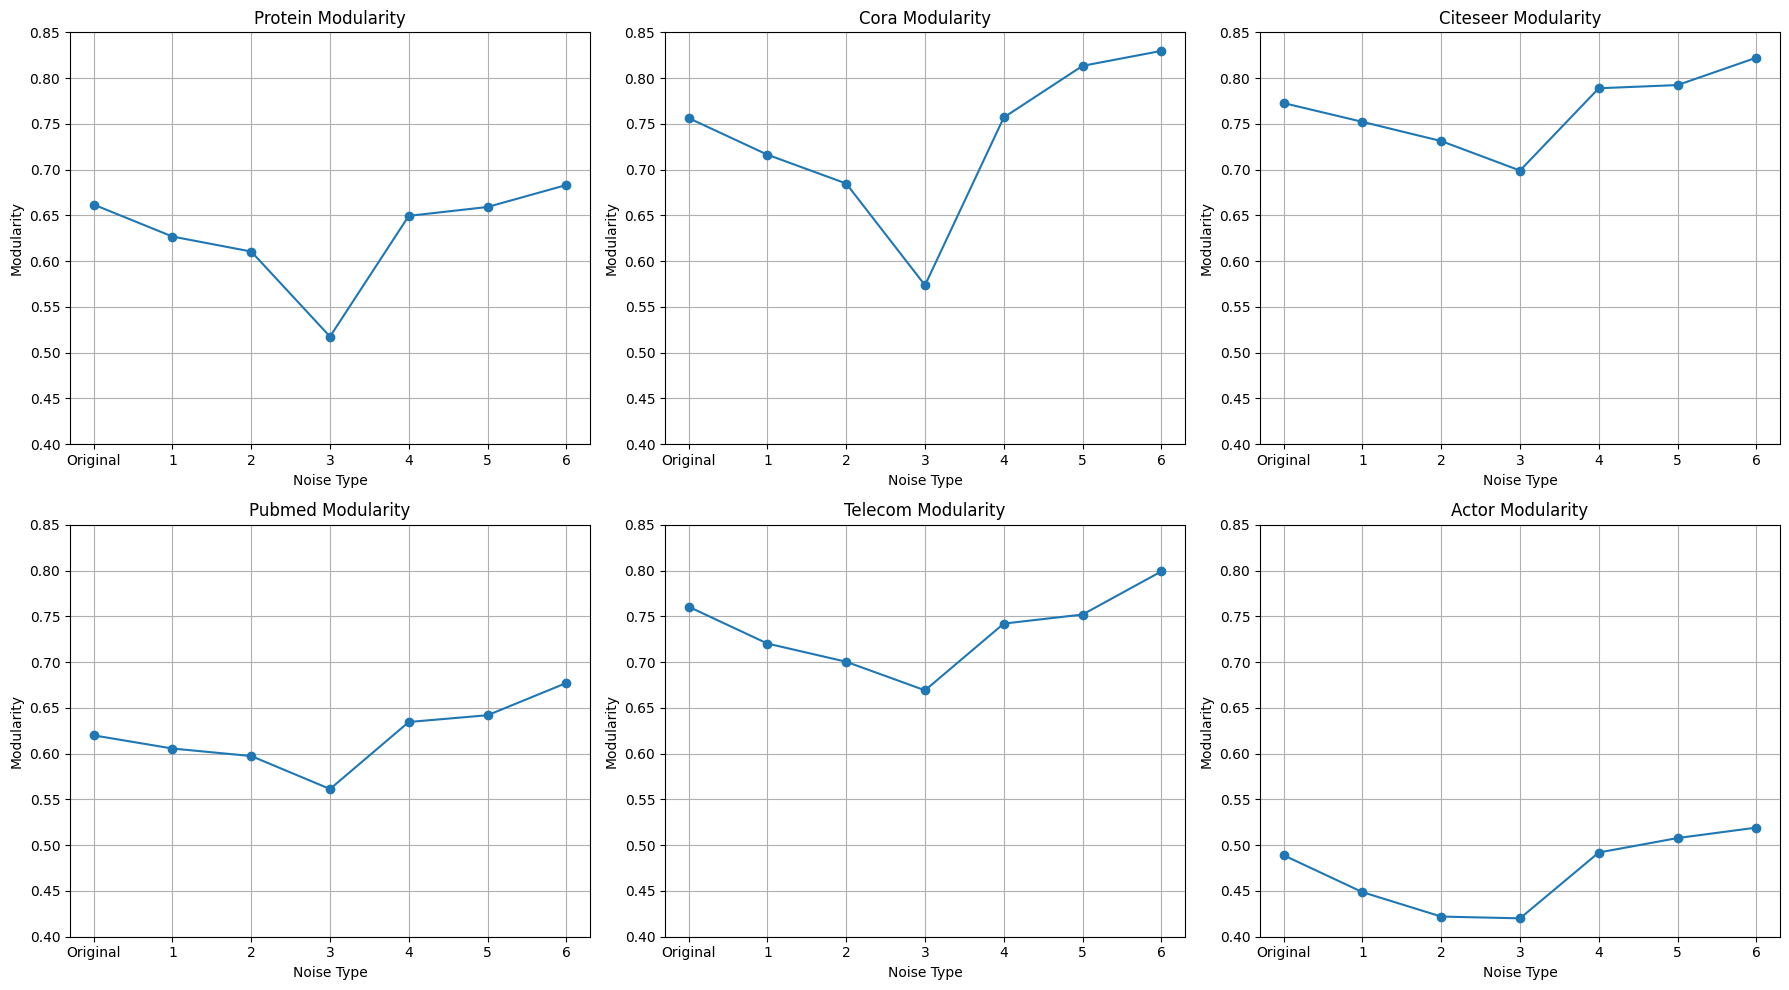
\includegraphics[width=0.8\textwidth]{Figure_17.png} % Adjust the width to scale the image
    \caption{Noise Experiments}
\end{figure}
From the experiment in Figure 5.10, we find that LEGC also has some robustness in noisy environments, but the modularity performance decreases significantly when the probability of adding edge noise is 0.3. However, we were surprised to find that modularity increased when some edges were removed to disrupt the graph's topology. We believe this is because after removing some important edges, the model's community structure became more apparent. 

Meanwhile, we find that graphs with a uniform PageRank distribution are less affected by noise interference, as uniform graphs are more difficult to disrupt community structures. As a social network, the Actor dataset has a more uniform distribution of PageRank, making it difficult for noise to disrupt its community structure.
\subsection{Remove Layers in Graph Neural Networks}

We need to adjust the number of layers in the model and observe the performance changes of LEGC to demonstrate the rationality of the model layer design in Section 4.4. In theory, graph neural networks should not be designed with too many layers, as \textbf{Over Smoothing} may occur. However, we still need to discuss the changes in model performance when GNN is one layer. If there is no significant change in model performance, we believe we can reduce the number of layers in the model instead of unthinkingly pursuing too deep models. We can calculate that the performance changes of GNNs with different layers are shown in Figure 5.11.
\begin{figure}[h] % 'h!' attempts to position the figure here
    \centering
    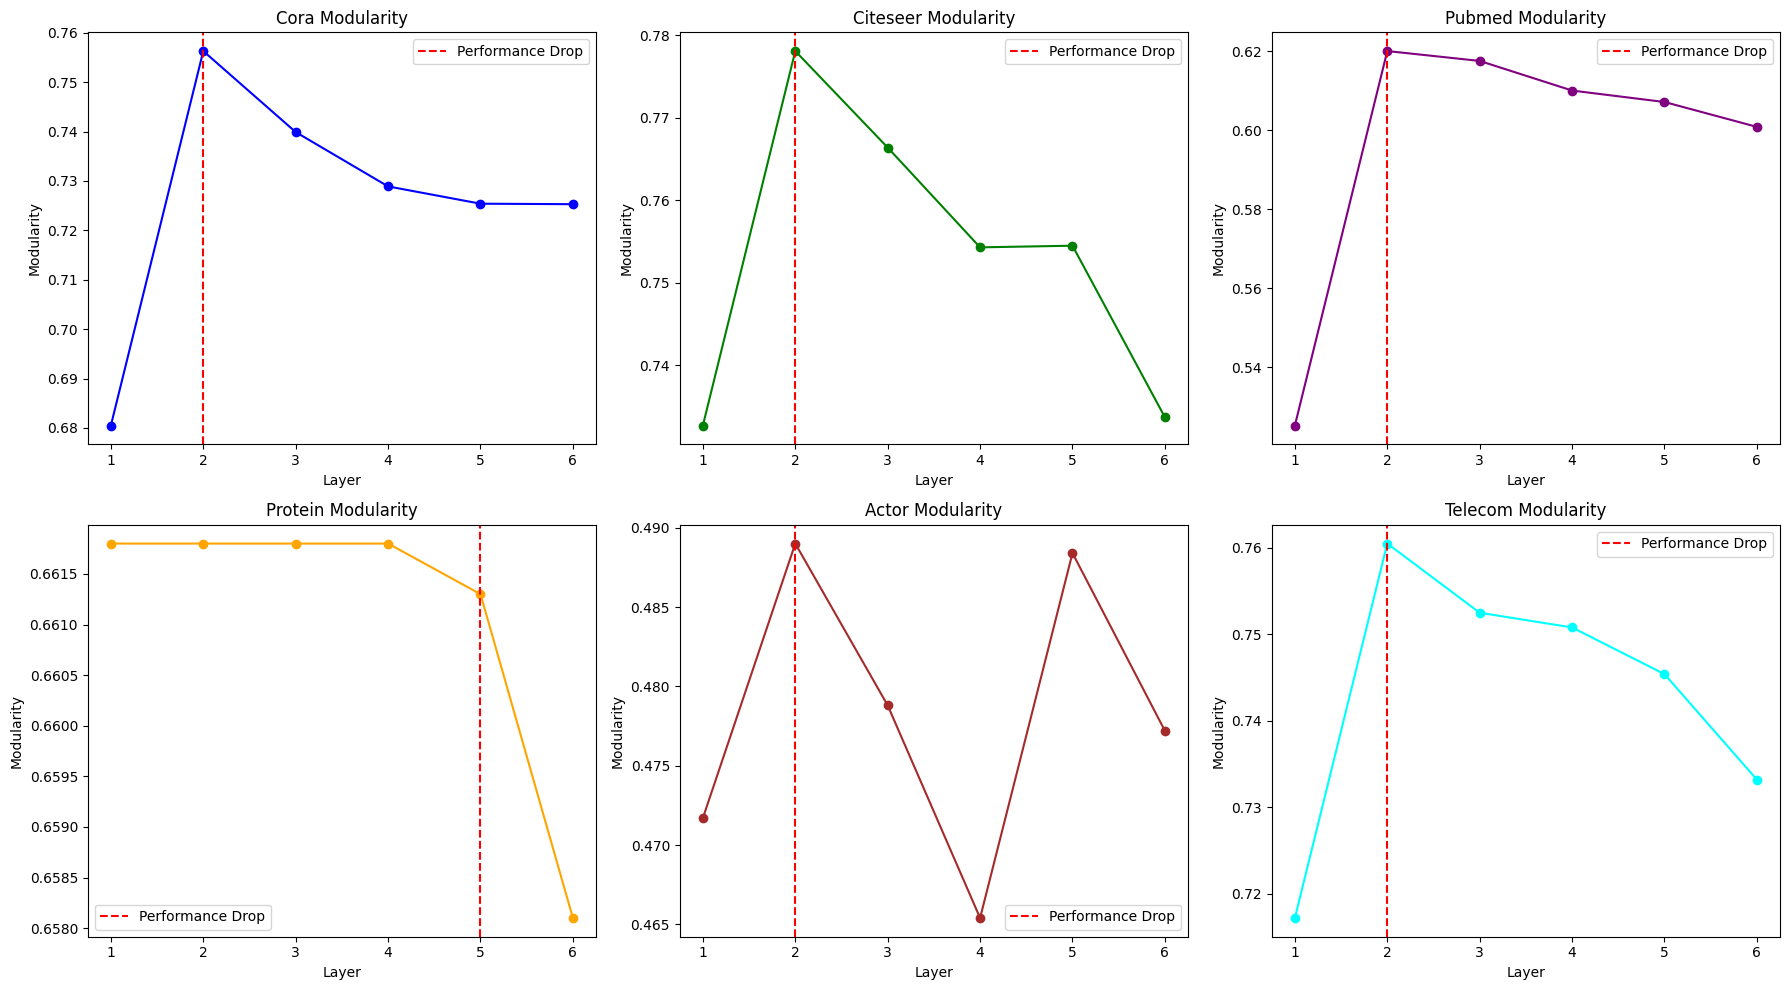
\includegraphics[width=0.8\textwidth]{Figure_18.png} % Adjust the width to scale the image
    \caption{ Performance Changes of GNNs with Different Layers}
\end{figure}
From Figure 5.11, we can conclude that we can achieve the same performance with a 1-layer GCN for small datasets. We need to use two or more layers of GCN to improve the model's ability to handle large datasets. However, when the number of layers exceeds 3, the model's performance still decreases due to \textbf{Over Smoothing}.



% -----------------------------------------------------------------------------

\chapter{Conclusion}
\label{chap:conclusion}
Chapter 6 briefly summarises our work and presents rigorous conclusions based on experimental results. In section 6.1, we introduce the status of our project and discuss whether our research objectives have been achieved, their degree of completion, and why some methods are not working. In section 6.2, we critically examine our model's limitations, and then in section 6.3, we identify our future work and model improvements based on the model's limitations.
\section{Project Status}
This dissertation proposes a novel community detection algorithm and applies it to Telecom Graphs and other datasets. It also provides commercial applications for community detection. Our proposed method of combining traditional community detection with ClusterNet (LEGC) has dramatically improved machine learning models' performance and training speed. 

We completed all the research aims mentioned in Section 1.3.1. For discussion, we listed the research aims of 1.3.1 as follows.
\begin{itemize}
\item Develop a community detection algorithm suitable for large-scale Telecom Graph data, providing insights into community detection for BT Research.
\item Explore the performance of different community detection algorithms and which are suitable for large-scale data.
\item Research whether using traditional community algorithms to enhance graph embedding vectors can improve machine learning algorithms' performance and training speed.
\item Compare the performance of different algorithms on different datasets.
\item Investigating whether graph community detection can label data and allow efficient and massively transformation of unsupervised datasets into supervised datasets.
\end{itemize}
For research aim 1, our model LEGC can effectively accelerate the training of large datasets and improve their performance. We conducted detailed comparisons and ablation experiments in Section 5.4. Meanwhile, in Section 5.3, we provide the usage of our community detection results, which include \textbf{Fault Detection}, \textbf{Network Environment Guarantee}, \textbf{Redundancy Planning}, \textbf{Personalized Application}, and \textbf{Micro Recommendation Systems}.

For research aim 2, we conducted a detailed comparison of the performance and time of different models in section 5.2. We provided algorithm frameworks for other models in section 1.2.2 to strengthen the theoretical basis of our conclusions. We conclude that using the traditional community algorithm Louvain for community detection is highly efficient when there is only structural information of the graph and no node and edge features. With node features and edge features, machine learning algorithms can be used to obtain more meaningful community partitioning. Meanwhile, we find that complex models may not necessarily perform well. For some datasets, using GCN and GraphSAGE is more efficient than Transformer. Therefore, when selecting a model, it is necessary to conduct experimental analysis based on the dataset.

For research aim 3, we conducted detailed experiments in Section 5.3 and concluded that traditional community detection algorithms can significantly improve graph neural networks' training speed and model performance.

For research aim 4, we used six graph datasets from various fields, including Telecom Graphs, and demonstrated their respective performance to demonstrate the robustness of our model and method.

For research aim 5, we calculated the NMI of the labels and community detection results of the supervised datasets. We find that the highest NMI between our community detection results and accurate labels was around \textbf{0.4}, which allows community detection methods to annotate data. Labelling large graph datasets is very time-consuming, and we can use community detection methods to provide labels for large graph datasets.
\section{Limitations}
Our model also has some limitations. Firstly, our machine learning method does not consider the existence of overlapping communities, where each node can only have one community. This algorithm has certain limitations. If users from both communities are enthusiastic about one package or application, then this package or application belongs to both communities simultaneously. Secondly, although our model excels in modularity compared to other scholars' models, our model performs worse on NMI than others. This may be due to other scholars using labels as training optimisation objectives. However, our model's performance on labelled data must be further adjusted and optimised to improve. Finally, due to the inconsistency of initialising cluster centres, the initial modularity of our model is not stable, and we need to specify the number of clusters in advance, which is challenging to execute in some cases. At the same time, the K-means algorithm is sensitive to outliers and may lose some model performance.
\section{ Future work}
Based on the limitations of our model, our future work is as follows.
\begin{itemize}
\item We can incorporate the algorithm BigCLAM~\cite{yang2013overlapping} for detecting overlapping communities into our model while taking the \textbf{Modularity of Overlapping Communities}~\cite{fortunato2007resolution} as the optimisation objective. We can improve our algorithm (LEGC) to BigCLAM Enhanced-GNN-Clusternet (BCEGC), which can detect overlapping communities.
\item Due to some drawbacks of K-means, the modularity of our model's initial epoch is not stable. We can use algorithms such as \textbf{Improved K-means~\cite{na2010research}} to enhance the stability of our model.


\item If the initial community detection results are too many, it will lead to too many features that need to be added and are relatively sparse. We can use some linear dimensionality reduction methods to convert one-hot representation larger than 50 dimensions into PCA representation to optimise our method further.

\item We need to increase the NMI performance of the model because it did not perform better than other scholars' models. We can change the optimisation objective from modularity to modularity+similarity of features within the same cluster. It enables our model to optimise modularity while placing nodes with similar features in the same community as much as possible. This approach will improve NMI, but the performance of modularity may deteriorate. So, choosing the best loss function is a significant direction for our future work.


\end{itemize}
\section{Suggestion}
Enterprises can use telecommunications graphs for user segmentation, precise marketing, and resource optimisation of base stations. However, it should be noted that the telecommunications map contains users' personal privacy information, and the divided communities also include the geographical information of each user. Enterprises need to comply with GDPR~\cite{voigt2017eu} strictly, obtain user consent, and ensure that the development of AI technology meets legal requirements when training and using models.





% =============================================================================

% Finally, after the primary matter, the back matter is specified.  This is
% typically populated with just the bibliography.  LaTeX deals with this % in one of two ways, namely
%
% - inline, which roughly means the author specifies entries using the 
%   \bibitem macro and typesets them manually BibTeX or
% - using BiBTeX, which means entries are contained in a separate file
%   (which is essentially a database) then imported; this is the 
 %   approach is used below, with the database being dissertation. bib.
%
% Either way, the each entry has a key (or identifier) which can be used
% in the main matter to cite it, e.g., \cite{X}, \cite[Chapter 2}{Y}.

\backmatter

\bibliography{sample_bibtex.bib}


% -----------------------------------------------------------------------------

% The dissertation concludes with a set of (optional) appendices; these are 
% the same as chapters in a sense, but once signalled as being appendices via
% the associated macro, LaTeX manages them appropriately.

\appendix

\chapter{GitHub Repository}
\label{appx:example}
GitHub Repository: https://github.com/TengyaoTu/Graph-Community-Detection



% =============================================================================

\end{document}
